\BourbakiExerciseGroup

\begin{enumerate}
\def\labelenumi{\arabic{enumi})}
\item
  设 \((x_{i})_{i\in I}\) 是完备豪斯多夫交换群 \(G\) 中的一个可和族，并设 \(\mathfrak{S}\) 是 \(I\) 的子集所成的一个集，它关于关系 \(\subset\) 有向，且构成 \(I\) 的一个覆盖。试证 \(\sum_{i\in I}x_{i} = \lim_{J}\sum_{i\in J}x_{i}\) ，其中极限是关于 \(\mathfrak{S}\) 的截面滤子取的。
\item
  设 G 是一个完备豪斯多夫交换群，使得 o 在 G 中的每个邻域都包含 G 的一个开子群（若 G 局部紧且全不连通，特别地即属此情形；参看 § 4 习题 18）。G 的点所成的族 \((x_{t})_{t\in I}\) 可和的充分必要条件是：关于 I 的有限子集的余集所成的滤子，\(\lim x_t = 0\) 。由此试证：G 中每个收敛级数都是交换收敛的。
\item
  设 \((x_{i})_{i\in I}\) 是豪斯多夫交换群 G 中点的一个族。对 I 的每个有限子集 H，令 \(s_{H}\) 表示 \(\sum_{i\in H}x_{i}\) ，而
\end{enumerate}

设 A 是映射 \(H \rightarrow s_{H}\) 关于有向集 \(\mathfrak{F}(I)\) 的诸聚点所成之集。对 I 的每个有限子集 J，令 \(\Phi(J)\) 表示诸点 \(s_{H}\) 所成之集的闭包，其中 H 取遍 I 中使 \(H \cap J = \varnothing\) 的有限子集。试证：若 \(A \neq \varnothing\) ，则集 A - A（即由所有 \(x - x'\) 组成的集，其中 \(x \in A\) 且 \(x' \in A\) ）与集 \(B = \bigcap_{J \in \mathfrak{F}(I)} \Phi(J)\) 相同；并且无论如何都有 \(B + B \subset B\) 。由此推出：若 A 非空，则 B 是 G 的一个闭子群，且 A 是 G 中 B 的一个陪集。

\begin{enumerate}
\def\labelenumi{\arabic{enumi})}
\setcounter{enumi}{3}
\item
  沿用习题 3 的记号，取 G 为有理整数组成的离散加法群 Z，取 I 为集合 N。试给出一个不可和序列 \((x_{n})\) 的例子，对于它集合 A 仅由单点 o 组成（选取诸 \(x_{n}\) ，使得每个其各项的指标都 \(\geqslant m\) 的有限部分和都是 m 的整数倍）。
\item
  设 \((x_{n})\) 是豪斯多夫交换群中点的一个序列。若对 N 的每个无限子集 I，由序列 \((x_{n})_{n\in I}\) 所定义的级数都收敛，则序列 \((x_{n})\) 是可和的（仿照命题 9 的证明，用反证法论证）。
\end{enumerate}

¶ 6) a) 设 \(\sigma\) 是 \(\mathbf{N}\) 的一个置换，并设 \(\varphi(n)\) 是 \(\mathbf{N}\) 中其并为 \(\sigma([0, n])\) 的区间的最小个数。假设 \(\varphi(n)\) 当 \(n\) 取遍 \(\mathbf{N}\) 时有界。那么，若 \((u_n)\) 是任一项都属于豪斯多夫交换群 \(\mathbf{G}\) 的收敛级数，则级数 \((u_{\sigma(n)})\) 收敛，且与 \((u_n)\) 有相同的和。

* b) 假设 \(\varphi(n)\) 在 N 中不有界。试构造一个级数 \((u_n)\) ，它的项都属于加法群 R，并且它在 R 中收敛，但级数 \((u_{\sigma(n)})\) 不收敛。{[}考虑一个严格递增的整数序列 \((m_k)\) ，它对 \(k\) 用归纳法定义，且满足下列条件：(i) 若 \([0, n_k]\) 是 N 的以 o 为左端点且包含于 \(\sigma([0, m_k])\) 的最大区间，则

\[
\sigma ([ 0, m _ {k} ]) \subset [ 0, n _ {k + 1} ];
\]

\begin{enumerate}
\def\labelenumi{(\roman{enumi})}
\setcounter{enumi}{1}
\tightlist
\item
  \(\varphi(m_k) \geqslant k + 1\) 。然后对 \(u_n\) 适当加以定义，其中 n 满足 \(n_k < n < n_{k+1}]\) 。试把上述结果推广到由 o 的每个邻域生成的完备豪斯多夫交换群 G 的情形。*
\end{enumerate}

\begin{enumerate}
\def\labelenumi{\arabic{enumi})}
\setcounter{enumi}{6}
\tightlist
\item
  设 \((x_{mn})\) 是豪斯多夫交换群 \(\mathbf{G}\) 中点的双重序列，满足下列条件：
\end{enumerate}

\begin{enumerate}
\def\labelenumi{(\alph{enumi})}
\item
  由序列 \((x_{mn})_{n\in \mathbb{N}}\) 所定义的级数对每个 \(m\geqslant 0\) 收敛；令 \(y_{m}\) 为其和。
\item
  若令 \(r_{mn} = \sum_{p=n}^{\infty} x_{mp}\) ，则由序列 \((r_{mn})_{m \in \mathbb{N}}\) 所定义的级数对每个 \(n \geqslant 0\) 收敛；令 \(t_n\) 为其和。
\end{enumerate}

试证：对每个 \(n \geqslant 0\) ，由序列 \((x_{mn})_{m \in \mathbb{N}}\) 所定义的级数收敛，并令 \(z_{n}\) 为其和。通项为 \(y_{m}\) 的级数与通项为 \(z_{n}\) 的级数有相同的和，当且仅当 \(t_{n}\) 当 n 趋于无穷时趋于 0。

\BourbakiExerciseGroup

\begin{enumerate}
\def\labelenumi{\arabic{enumi})}
\item
  在豪斯多夫拓扑环 A 中，A 的每个子集的中心化子（特别地，A 的中心）是闭的，并且 A 的每个子集的左（相应地，右）零化子也是闭的。
\item
  \begin{enumerate}
  \def\labelenumii{\alph{enumii})}
  \tightlist
  \item
    设 \(\mathfrak{a}\) 是拓扑环 A 中的离散左理想。试证：对每个 \(x \in \mathfrak{a}\) ，\(x\) 在 A 中的左零化子是开的。由此试证：若 A 是无非零因子的非离散环，则它不含 \(\{\mathbf{o}\}\) 以外的离散（左或右）理想。
  \end{enumerate}
\end{enumerate}

\begin{enumerate}
\def\labelenumi{\alph{enumi})}
\setcounter{enumi}{1}
\tightlist
\item
  设 A 是局部连通拓扑环，\(\mathfrak{a}\) 是 A 的全不连通左理想。试证：对每个 \(x \in \mathfrak{a}\) ，\(x\) 在 A 中的左零化子是开的。由此试证：若 A 无零因子，则它不含 \(\{0\}\) 以外的全不连通（左或右）理想。
\end{enumerate}

\begin{enumerate}
\def\labelenumi{\arabic{enumi})}
\setcounter{enumi}{2}
\item
  拓扑环 A 中 o 的连通分支是双边理想。由此推出：若 A 是拟单的且不连通（特别地，若 A 是不连通的拓扑除环），则 A 全不连通。
\item
  设 \((x_{i})\) 是豪斯多夫拓扑环 A 中的可和族，\(s\) 为其和。则对每个 \(a \in A\) ，族 \((ax_{i})\){[}相应地 \((x_{i}a)]\)可和，且其和为 as（相应地，sa）。若 \((x_{\lambda})\) 与 \((y_{\mu})\) 是 A 中两个可和族，且族 \((x_{\lambda}y_{\mu})\) 可和，则 \(\sum_{\lambda,\mu} x_{\lambda} y_{\mu} = \left( \sum_{\lambda} x_{\lambda} \right) \left( \sum_{\mu} y_{\mu} \right)\) 。此外，若 A 完备且诸 \(x_{\lambda}\) 之一是可逆元，则族 \((x_{\lambda}y_{\mu})\) 的可和性蕴含 \((y_{\mu})\) 的可和性。
\item
  矩形是 \(N \times N\) 的一个子集，它是 N 的两个区间的乘积。给定 \(N \times N\) 的有限子集 E，令 \(\varphi(E)\) 为其并为 E 的两两不相交矩形的最小个数。设 \((E_n)\) 是 \(N \times N\) 的有限子集的一个递增序列，它覆盖 \(N \times N\) ，且使序列 \((\varphi(E_n))\) 有界。若 \((x_n), (y_n)\) 是两个收敛级数，其项都属于豪斯多夫拓扑环 A，则我们有
\end{enumerate}

\[
\lim _ {n \rightarrow \infty} \sum_ {(h, k) \in \mathrm{E} _ {n}} x _ {h} y _ {k} = \left(\underset {n = 0} {\overset {\infty} {\sum}} x _ {n}\right)\left(\underset {n = 0} {\overset {\infty} {\sum}} y _ {n}\right).
\]

试构造一个满足上述条件的序列 \((\mathbf{E}_{n})\) 的例子，使得对每个 n，\(E_{n+1} - E_{n}\) 只含一个元素。

\begin{enumerate}
\def\labelenumi{\arabic{enumi})}
\setcounter{enumi}{5}
\item
  设 A 是有单位元的拓扑环，\(a, b\) 是 A 的两个双边理想，满足 \(a + b = A\) 且 \(a \cap b = \{0\}\) 。试证拓扑环 A 同构于拓扑环 a 与 b 的乘积。
\item
  设 A 是无单位元的拓扑环，B 是由 A 添加一个单位元而得到的环。试证：B 上由 A 的拓扑与 Z 上离散拓扑的乘积所成的拓扑与 B 的环结构相容，并且在 A（B 的一个双边理想）上诱导出所给的拓扑。
\item
  设 \(\mathbf{A}\) 是有单位元的拓扑环。
\end{enumerate}

\begin{enumerate}
\def\labelenumi{\alph{enumi})}
\item
  A 的可逆元所成的集 A* 在 A 中是开的，当且仅当存在 1 的一个邻域 V，它的所有元素都是 A 的可逆元。
\item
  若 A* 在 A 中是开的，则 A 的每个极大（左或右）理想都是闭的，并且 A 的根基是闭的。若 A 除 \(\{o\}\) 与 A 外没有其他闭左理想，则 A 是一个除环。
\item
  设 A 是拓扑域 Q 中由所有有理数 \(k/2^{n}\) （ \(k \in Z, n \in N\) ）组成的子环。试证 A 不含 \(\{0\}\) 与 A 以外的闭理想，但 A 不是域。
\end{enumerate}

\begin{enumerate}
\def\labelenumi{\arabic{enumi})}
\setcounter{enumi}{8}
\tightlist
\item
  \begin{enumerate}
  \def\labelenumii{\alph{enumii})}
  \tightlist
  \item
    元素 \(x\) （相应地，理想 \(\mathfrak{a}\) ）称为拓扑环 \(\mathbf{A}\) 中的拓扑幂零元，如果序列 \((x^n)_{n\geqslant 1}\) 收敛于 o {[}相应地，如果由诸 \(\mathfrak{a}^n\) （ \(n\geqslant 1\) ）组成的滤子基收敛于 o）。拓扑幂零理想的每个元素都是拓扑幂零的。
  \end{enumerate}
\end{enumerate}

\begin{enumerate}
\def\labelenumi{\alph{enumi})}
\setcounter{enumi}{1}
\item
  假设 A 有单位元，且 \(A^{*}\) 在 A 中是开的。试证：若 x 是 A 的任一拓扑幂零元素，则 1 - x 是可逆元（注意，当 n 充分大时 \(1 - x^{n}\) 是可逆元）。由此试证：若（左或右）理想 a 的所有元素都是拓扑幂零的，则 a 包含在 A 的根基中。
\item
  假设 A 完备且有单位元，并且存在由 A 的加法群的子群组成的 o 的基本邻域系。试证：若 x 拓扑幂零，则 1 - x 是 A 中的可逆元。
\end{enumerate}

\(d)\) 在 \(c\) ) 的假设下，试证：若 \(y \in A\) 拓扑幂零，则方程 \(x^{2} + x = y\) 有一个根 \(x \in A\) ，并且 \(x\) 拓扑幂零。

¶ 10) a) 设 B 是有单位元的环，E 是自由 B-模 \(\mathbf{B}_{d}^{(I)}\) ，A 是 E 的自同态环 \(\mathcal{L}(\mathbf{E})\) 。对 E 的每个有限子集 F，令 \(V_{F}\) 为所有这样的 \(u \in A\) 组成的集：\(u(x) = 0\) 对所有 \(x \in F\) 成立。试证诸 \(V_{F}\) 构成 A 上某个豪斯多夫拓扑的 o 的基本邻域系，该拓扑与 A 的环结构相容，且对此拓扑 A 全不连通。

\begin{enumerate}
\def\labelenumi{\alph{enumi})}
\setcounter{enumi}{1}
\tightlist
\item
  取 I = N，并取 B 为一个没有零因子但其根基 R 不是 \(\{0\}\) 的交换环。试证 A 的根基不是闭的。{[}设 \((e_{n})\) 是 E 的典范基。一方面注意：每个 \(u \in A\) ，只要它除有限多个指标外都有 \(u(e_{n}) = 0\) ，且 \(u(E) \subset \Re \cdot E\) ，就属于 A 的根基；另一方面考察 A 的如下元素 \(u_{0}\) ：\(u_{0}(e_{n}) = e_{n} + te_{n+1}\) （其中 \(t \neq 0\) 属于 R，对每个 n）{]}。
\end{enumerate}

¶ 11) a) 有单位元的拓扑环称为 Gelfand 环，如果 A* 在 A 中是开的，并且 A 的拓扑在 A* 上诱导的拓扑与 A* 的乘法群结构相容。每个豪斯多夫拓扑除环都是 Gelfand 环{[}参看习题 20 e){]}。

\begin{enumerate}
\def\labelenumi{\alph{enumi})}
\setcounter{enumi}{1}
\tightlist
\item
  试证：若 A 是 Gelfand 环，则每个赋有乘积拓扑的矩阵环 \(\mathbf{M}_{n}(\mathbf{A})\) （乘积拓扑取在 \(A^{n^{2}}\) 上）也是 Gelfand 环。（对 n 用归纳法证明。）
\end{enumerate}

\begin{enumerate}
\def\labelenumi{\arabic{enumi})}
\setcounter{enumi}{11}
\tightlist
\item
  拓扑环的子集 M 称为右有界的（相应地，左有界的），如果对 A 中 o 的每个邻域 U，存在 o 的邻域 V 使 VM⊂U（相应地，MV⊂U）；若 M 既左有界又右有界，则称 M 为有界的。若 A 中存在 o 的有界邻域，则称 A 的拓扑是局部有界的（且称 A 为局部有界拓扑环）。
\end{enumerate}

\begin{enumerate}
\def\labelenumi{\alph{enumi})}
\item
  每个具有由右理想组成的 o 的基本邻域系的拓扑环都是右有界的。试证：在习题 10 a) 中，若 I 无限且 B 是除环，则环 A 是左有界的，但 A 中不存在 o 的右有界邻域。
\item
  若拓扑环 A 是右有界的（相应地，有界的），且具有由 A 的加法群的子群组成的 o 的基本邻域系，则它具有由右（相应地，双边）理想组成的 o 的基本邻域系。
\item
  有界集的每个有限并是有界的；有界集的闭包是有界的；若 M 与 N 有界，则 \(M + N\) 与 MN 也有界。
\item
  拓扑环 \(\mathbf{A}\) 中的每个准紧集是有界的。
\item
  若 M 与 N 是 A 的两个有界子集，试证映射 \((x, y) \to xy\) （把 \(M \times N\) 的元素映入 A）是一致连续的。
\item
  设 A 是有单位元的豪斯多夫拓扑环。试证：若 \((x_{n})\) 是 A 中趋于 o 的可逆元序列，则诸元素 \(x_{n}^{-1}\) 所成之集既非左有界也非右有界。
\item
  若 A 是有单位元的有界环，试证映射 \(x \rightarrow x^{-1}\) 在 A 的可逆元集 A* 上是一致连续的。h) 试证：若 A 是有单位元的完备豪斯多夫有界环，则可逆元集 A* 与 A 的根基都是闭的{[}利用 g){]}。
\item
  拓扑环的乘积 \(\prod_{t} A_{t}\) 的子集是有界的，当且仅当它的所有投影都是有界的。
\item
  局部有界环的每个子环以及局部有界环的每个乘积都是局部有界环。
\item
  局部有界豪斯多夫环的完备化是局部有界的。
\end{enumerate}

\begin{enumerate}
\def\labelenumi{\arabic{enumi})}
\setcounter{enumi}{12}
\tightlist
\item
  设 A 是有界拓扑环（习题 12），它有单位元，并且 A 的可逆元集 A* 在 A 中是开的。试证 A 的根基是开的。因此，若 A 无根基，则它是离散的；特别地，有界豪斯多夫拓扑除环是离散的。无根基、有单位元且 A* 为开的紧环 A 是有限的；特别地，紧拓扑除环是有限的。
\end{enumerate}

¶ 14) 设 A 是全不连通（*）、无根基且有单位元的紧环。则 A 同构于一个有限单环族的乘积。{[}首先利用 § 6 习题 12 b) 与 § 4 命题 14 证明：A 具有由双边理想组成的 o 的基本邻域系。然后证明存在 A 的双边理想的一个极大集 \(\Phi\) ，使得：(i) 每个双边理想 \(\mathfrak{M} \in \Phi\) 都是 A 的极大开双边理想；(ii) 没有理想 \(\mathfrak{M} \in \Phi\) 包含 \(\Phi\) 中异于 \(\mathfrak{M}\) 的理想的有限交。再证明 A 同构于诸环 \(A/\mathfrak{M}\) （ \(\mathfrak{M}\) 取遍 \(\Phi\) ）的乘积；先利用习题 9 b) 证明所有 \(\mathfrak{M} \in \Phi\) 的交仅由 A 的零元素组成{]}。
(*) 可以证明，有单位元的紧环必然全不连通。

\begin{enumerate}
\def\labelenumi{\arabic{enumi})}
\setcounter{enumi}{14}
\item
  设 A 是全不连通且有单位元的紧环。试证 A 的根基 \(\Re\) 是拓扑幂零的{[}习题 9 a)；利用 § 6 习题 12 b) 与 § 4 命题 14{]}。由此试证 \(\Re\) 是由所有这样的 \(x \in A\) 组成的集：\(ax\) 对每个 \(a \in A\) 都拓扑幂零{[}参看习题 9 c){]}。
\item
  试证：在环 A（相应地，除环 K）上，\(\mathcal{C}\) （与 A 的环结构（相应地，K 的除环结构）相容的一族拓扑 \((\mathcal{T}_i)\) 的上确界）与该结构相容。对拓扑 \(\mathcal{T}_i\) 中的每一个都左（相应地，右）有界的集 M，对 \(\mathcal{C}\) 也左（相应地，右）有界。
\item
  若 K 是非离散的豪斯多夫拓扑除环，则 K 上的两个乘法一致结构没有一个能与 K 的加法一致结构在 \(K^{*}\) 上诱导的一致结构相比较（参看习题 13）。
\item
  设 K 是豪斯多夫拓扑除环，A 是 K 的闭子集，B 是 K 的紧子集且 \(o \notin B\) 。试证 AB 与 BA 在 K 中是闭的（参看 § 4 第 1 目命题 1 推论 1）。* 在实数域 R 中，给出一个例子，其中 A 是闭的，B 是紧的，\(o \in B\) ，而 AB 不是闭的。*
\item
  \begin{enumerate}
  \def\labelenumii{\alph{enumii})}
  \tightlist
  \item
    设 K 是赋有与 K 的环结构相容的豪斯多夫拓扑 \(\mathcal{G}\) 的除环。试证：K 中存在 o 的邻域 V，使 \((\mathbb{CV}) \cup (\mathbb{CV})^{-1} = \mathbf{K}^*\) {[}这等价于 \(\mathbf{V} \cap (\mathbf{V} \cap \mathbf{K}^*)^{-1} = \emptyset\) {]}。
  \end{enumerate}
\end{enumerate}

\begin{enumerate}
\def\labelenumi{\alph{enumi})}
\setcounter{enumi}{1}
\tightlist
\item
  再假设 \(\mathfrak{C}\) 不是离散的。试证：若 \(\mathbf{U}\) 是 \(o\) 在 \(\mathbf{K}\) 中的任一邻域，且 \(\mathbf{U}^*\) 表示 \(\mathbf{U} \cap \mathbf{K}^*\) ，则
\end{enumerate}

\[
\mathbf {U} ^ {*} (\mathbf {U} ^ {*}) ^ {- 1} = \mathbf {K} ^ {*}.
\]

¶ 20) a) 设 K 是赋有与 K 的环结构相容的非离散豪斯多夫拓扑 \(\mathfrak{C}\) 的除环。K 的子集 M 是右（相应地，左）有界的，当且仅当对 o 的每个邻域 U，存在 \(a \in \mathbf{K}^*\) 使 \(a\mathbf{M} \subset \mathbf{U}\) （相应地，Ma \(\subset\) U）；此时，M 对每个豪斯多夫拓扑 \(\mathfrak{C}'\) （它比 \(\mathfrak{C}\) 粗且与 K 的环结构相容）都是右（相应地，左）有界的。

\begin{enumerate}
\def\labelenumi{\alph{enumi})}
\setcounter{enumi}{1}
\item
  若 \(\mathfrak{G}\) 是局部有界的（习题 12），且 U 是关于 \(\mathfrak{G}\) 的 o 的有界邻域，则诸集 \(x\mathrm{U}\) （相应地，\(\mathrm{U}x\) ）构成 o 的（关于 \(\mathfrak{G}\) 的）基本邻域系，这里 x 取遍 \(\mathbf{K}^*\) 。K 的每点具有关于 \(\mathfrak{G}\) 的可数基本邻域系，当且仅当存在以 o 为聚点的 K 中的点列 \((a_n)\) 。
\item
  K 上局部有界拓扑（与 K 的环结构相容的）的任一有限族的上确界是局部有界的。反之，设 \(\mathcal{G}\) 是 K 上局部有界拓扑的某个族 \((\mathfrak{T}_i)\) 的上确界；若它局部有界，则 \(\mathcal{G}\) 是 \((\mathfrak{T}_i)\) 的某个有限子族的上确界。（注意：若 U 是关于 \(\mathcal{G}\) 有界的 o 的邻域，则存在有限的指标组 \((\iota_k)\) ，并且对每个 \(k\) 存在 o 的邻域 \(\mathrm{V}_k\) （它关于 \(\mathcal{G}_{\iota_k}\) 有界），使 \(\bigcap \mathrm{V}_k \subset \mathrm{U}\) ；另一方面，存在 \(a_k \in \mathrm{K}^*\) 使 \(\mathrm{U} \subset a_k \mathrm{V}_{k'}\) 。）
\item
  除环 K 的子集 F 称为拟环，如果：(i) \(F \neq K\) ，\(o \in F\) ，\(1 \in F\) ，\(-F = F\) ，\(FF \subset F\) ；(ii) 存在元素 \(c \in F^{*} = F \cap K^{*}\) 使 \(c(F + F) \subset F\) ；并且 (iii) 对每个 \(x \in F\) ，存在 \(y \in F\) 使 \(yF \subset Fx\) 且 \(Fy \subset xF\) 。试证：若 G 是局部有界且与 K 的环结构相容的非离散豪斯多夫拓扑，则 o 的每个满足 \(UU \subset U\) 且 \(1 \in U\) 的（关于 G 的）对称有界邻域 U 都是拟环，并且 \(U^{*}(U^{*})^{-1} = K^{*}\) {[}习题 19 b){]}。若 V 是关于 G 的 o 的任一对称有界邻域，则由诸元素 \(x \in K\) （它们满足 \(xV \subset V\) ，或 \(Vx \subset V\) ）组成的集 U 是关于 G 的 o 的对称有界邻域，它满足 \(UU \subset U\) 且 \(1 \in U\) ，因而是拟环。
\item
  反之，设 F 是 K 中满足 \(\mathrm{F}^{*}(\mathrm{F}^{*})^{-1} = \mathrm{K}^{*}\) 的拟环。试证：存在非离散且与 K 的环结构相容的豪斯多夫拓扑 G，使 F 是关于 G 的 o 的有界邻域。特别地，可取 F 为 K 的任一子环 A，使 K 是 A 的右分式除环。特别地，若 K = Q 且 F = Z，则 K 上相应的拓扑 G 与 K 的域结构不相容。
\end{enumerate}

¶ 21) a) 设 \(\mathfrak{C}\) 是除环 K 上的局部有界豪斯多夫拓扑，对此拓扑 K 是连通的。试证 K 中存在非零的拓扑幂零元素{[}习题 9 a){]}。（若 U 是 o 的对称有界邻域，t 是 K 中使 \(\mathrm{U}t + t\mathrm{U} \subset \mathrm{U}\) 的非零元素，试利用 § 2 第 2 目命题 6 证明 K 是诸集 \(\mathrm{U}t^{-n}\) 的并。）

\begin{enumerate}
\def\labelenumi{\alph{enumi})}
\setcounter{enumi}{1}
\tightlist
\item
  设 \(\mathfrak{G}\) 是 K 上的局部有界豪斯多夫拓扑，对此拓扑 K 有非零的拓扑幂零元素。试证：存在 o 的邻域 U，使得对 o 的每个邻域 V，存在整数 \(n_0\) ，使得 \(\mathrm{U}^n\subset \mathrm{V}\) 对所有 \(n\geqslant n_0\) 成立；这蕴含 U 的所有元素都拓扑幂零，并且 K 的每点具有关于 \(\mathfrak{G}\) 的可数基本邻域系。（设 \(t\neq 0\) 拓扑幂零，W 是 o 的有界邻域；取 U 为满足 \(\mathrm{UW}\subset \mathrm{Wt}\) 的 o 的有界邻域。）因此，K 的拓扑幂零元素所成之集 T 是关于 \(\mathfrak{G}\) 的 o 的邻域。
\end{enumerate}

¶ 22) 在赋有与 K 的环结构相容的豪斯多夫拓扑 \(\mathfrak{G}\) 的除环 K 中，包含 o 的集 R 称为逆有界的，如果 \((\mathbb{C}R)^{-1}\) 是有界的。若 K 中存在关于 \(\mathfrak{G}\) 的由 o 的逆有界邻域组成的基本系，则称 \(\mathfrak{G}\) 是局部逆有界的。

\begin{enumerate}
\def\labelenumi{\alph{enumi})}
\item
  局部逆有界的拓扑 T 是局部有界的，并且是所有与 K 的环结构相容的豪斯多夫拓扑所成之集中的一个极小元素；此外，C 与 K 的除环结构相容{[}利用习题 19 a){]}。
\item
  在本习题中从此假设 \(\mathcal{G}\) 是 K 上的局部逆有界拓扑。试证：对 K 中 o 的每个邻域 V，\(x \to x^{-1}\) 在 \(\mathbb{C}\mathrm{V}\) 上是一致连续的。由此试证 K 的完备化 \(\hat{\mathbf{K}}\) 是一个拓扑除环，其拓扑是局部逆有界的。
\item
  K 中 o 的每个邻域（关于 \(\mathfrak{G}\) 的）都包含 o 的一个邻域 V，使 \(\mathbf{E}(\mathbf{V}) = (\mathbb{C}\mathbf{V}) \cap (\mathbb{C}\mathbf{V})^{-1}\) 非空。试证：由 K 的加法一致结构与两个乘法一致结构在 \(\mathbf{E}(\mathbf{V})\) 上诱导的三个一致结构重合。由此推出：若 K 完备，则 \(\mathbf{K}^*\) 关于每个乘法一致结构都是完备的。
\item
  试证：若 \(x\) 是 \(\mathbf{K}^*\) 的元素，则下列三个命题中恰有一个为真：(i) \(x\) 拓扑幂零；(ii) \(x^{-1}\) 拓扑幂零；(iii) 序列 \((x^n)_{n\in \mathbb{Z}}\) 有界。{[}通过考察某个有界邻域 \(U\) ，它包含 \(o\) 且满足 \(UU\subset U\) （习题 20 d)），证明：若 o 是序列 \((x^n)_{n\geqslant 0}\) 的聚点，则 \(x\) 拓扑幂零。{]}若 K 含非零的拓扑幂零元素，试证：由 o 与所有这样的 \(x\in \mathbf{K}^*\) （ \(x^{-1}\) 不拓扑幂零）组成的集 B，是 K 中 o 的有界邻域，并且在所有内自同构下不变{[}利用习题 21 b){]}；于是 B 包含所有满足 \(\mathrm{UU}\subset \mathrm{U}\) 的 o 的有界邻域 U；这类在所有内自同构下不变的邻域所成之集有一个最大元素，当 \(\mathbf{K}^*\) 的换位子群有界时，特别地当 K 是域时，它与 B 重合。
\item
  若 U 是 K 中 o 的有界对称邻域且 \(UU \subset U\) ，则存在 \(b \in U^{*}\) 使 \(\mathbf{K}^{*} = \mathbf{U}^{*} \cup ((\mathbf{U}^{*})^{-1} b)\) 。设 \(a \in U^{*}\) 满足 \(Ua \subset bU\) ，并假设序列 \((a^{-n})_{n \geqslant 0}\) 有界。试证：由所有这样的 \(x \in K\) 组成的集 V：xU 包含于诸集 \(Ua^{-n}\) 的并之中，是 o 的有界邻域，满足 \(VV \subset V\) 且 \(\mathbf{K}^{*} = \mathbf{V}^{*} \cup (\mathbf{V}^{*})^{-1}\) 。
\item
  假设 K 不含非零的拓扑幂零元素。试证：K 中存在 o 的有界邻域，它是 K 的子环 A，且使 \(\mathbf{K}^{*} = \mathbf{A}^{*} \cup (\mathbf{A}^{*})^{-1}\) 。{[}从满足 \(\mathbf{K}^{*} = \mathbf{V}^{*} \cup (\mathbf{V}^{*})^{-1}\) 的 o 的有界邻域 V 出发（见 e){]}；若 \(c \in V^{*}\) 满足 \(c(V + V) \subset V\) ，则注意由 V 生成的环 A 包含于诸集 \(Vc^{-n}\) （ \(n \geqslant 0\) ）的并之中。
\end{enumerate}

¶ 23) 若 p 是任一素数，x 是任一非零有理数，令 \(v_{p}(x)\) 表示 p 在 x 的素因子分解中的指数。\(v_{p}\) 从 \(Q^{*}\) 到 Z 中的映射称为 Q 上的 p 进赋值。由所有这样的 \(x \in Q\) 组成的集：x = 0 或 \(v_{p}(x) \geqslant m\) （对某个 \(m \in Z\) ），是 Q 的分式理想 ( \(p^{m}\) )。

\begin{enumerate}
\def\labelenumi{\alph{enumi})}
\tightlist
\item
  试证：诸理想 \((p^{m})\) （ \(m \in Z\) ）构成 Q 中 o 关于某个局部逆有界拓扑（习题 22）\(C_{p}\) 的基本邻域系，该拓扑称为 p 进拓扑。Q 在此拓扑下的完备化 \(Q_{p}\) 是一个域，称为 p 进数域，其元素称为 p 进数。Z 的闭包 \(Z_{p}\) （在 \(Q_{p}\) 中）是 \(Q_{p}\) 中的一个紧开主理想整环，其中 \(p = pZ_{p}\) 是唯一的非零素理想；\(Z_{p}/p\) 同构于素域 \(F_{p} = Z/(p)\) ，并且更一般地，加法商群 \(p^{m}/p^{n}\) 同构于
\end{enumerate}

\[
\mathbf {Z} / (p ^ {n - m}) \text {   if   } m <   n.
\]

\(\mathbf{Z}_p\) 的元素称为 \(p\) 进整数。

\begin{enumerate}
\def\labelenumi{\alph{enumi})}
\setcounter{enumi}{1}
\item
  试证：加法群 \(Q_{p}\) 到其自身的每个连续同态都具有 \(x \to ax\) 的形式，其中 \(a \in Q_{p}\) {[}若 f 是这样一个同态，试证 \(f(rx) = rf(x)\) 对所有 \(r \in Q\) 成立，然后在 \(Q_{p}\) 中取极限{]}。
\item
  试证：每个紧子群 \(G \neq \{o\}\) （ \(Q_{p}\) 的加法群的子群）都与某个 \(p^{n} (n \in Z)\) 相同，并且加法群 \(Q_{p}\) 除 \(Q_{p}\) 自身外没有非紧的闭子群。{[}设 m 是使 \(G \subset p^{m}\) 的最大整数；通过考察商群 \((G + p^{n})/p^{n}\) （当 n \textgreater{} m 时），证明 \(G + p^{n} = p^{m}\) ，然后利用 § 3 第 1 目的公式 (1){]}。
\end{enumerate}

¶ 24) a) 试证：乘法群 \(\mathbf{Q}_p^*\) （ \(p\) 进数域 \(\mathbf{Q}_p\) 的乘法群）的每个子群都同构于乘法群 \(\mathbf{U}\) （ \(\mathbf{Z}_p\) 的可逆元的乘法群）的一个子群与一个同构于 \(\mathbf{Z}\) 或 \(\{o\}\) 的离散加法子群的乘积。

\begin{enumerate}
\def\labelenumi{\alph{enumi})}
\setcounter{enumi}{1}
\item
  试证：U 的子群 \(V = 1 + p\) 的紧子群就是诸群 \(1 + p^{n}\) {[}推理与习题 23 c) 的相同{]}。
\item
  试证：对每个 \(a \in \mathbf{U}\) ，序列 \((a^{p^n})_{n \in \mathbb{N}}\) 趋于一个极限 \(\alpha \equiv a \pmod{\mathfrak{p}}\) ，并且 \(\alpha^p = \alpha\) {[}证明 \(a^{p^n} \equiv a^{p^{n-1}} \pmod{\mathfrak{p}^n}\) （对 \(n\) 用归纳法）{]}。试证：多项式 \(\mathbf{X}^{p-1} - 1\) （在 \(\mathbf{Q}_p\) 的一个代数闭扩张中）的所有根都属于 \(\mathbf{Q}_p\) ，并且模 \(\mathfrak{p}\) 两两不同余{[}把前面所述应用于同余式 \(x^{p-1} - 1 \equiv 0 \pmod{p}\) 的根{]}。若 \(p > 2\) 且 \(d\) 是 \(n\) 与 \(p - 1\) 的最大公因子，则多项式 \(\mathbf{X}^n - 1\) 恰有 \(d\) 个根（在 \(\mathbf{Q}_p\) 中），它们都是 \(\mathbf{X}^d - 1\) 的根（同样的方法：取 \(a\) 为 \(\mathbf{X}^n - 1\) 的一个根）。
\end{enumerate}

由此试证：若 \(p > 2\) ，则乘法群 \(\mathbf{Q}_p^*\) 的每个紧子群都是 \(\mathbf{U}\) 的一个有限子群{[}由 \((p - 1)\) 次单位根组成{]}与一个形如 \(1 + \mathfrak{p}^n\) 的子群的直积{[}利用 \(b\){]}。当 \(p = 2\) 时这些结果应如何修改？（让群 \(1 + \mathfrak{p}^2\) 起先前由 \(1 + \mathfrak{p}\) 所起的作用。）

\begin{enumerate}
\def\labelenumi{(\arabic{enumi})}
\setcounter{enumi}{24}
\tightlist
\item
  \begin{enumerate}
  \def\labelenumii{\alph{enumii})}
  \tightlist
  \item
    设 \(a \neq o\) 是一个 \(p\) 进数。则映射 \(n \to a^n\) 在 \(\mathbf{Z}\) 上（作为 \(\mathbf{Q}_p\) 的子空间）连续，当且仅当 \(a \in 1 + \mathfrak{p}\) 。若此条件满足，试证 \(n \to a^n\) 在 \(\mathbf{Z}\) 上一致连续，并且可延拓为 \(\mathbf{Z}_p\) 到 U 中的连续同态，记作 \(x \to a^x\) ，当 \(a \neq 1\) 时它是单射。若 \(p > 2\) 且 \(m\) 是使 \(a \in 1 + \mathfrak{p}^m\) 的最大整数，则 \(x \to a^x\) 是 \(\mathbf{Z}_p\) 到 \(1 + \mathfrak{p}^m\) 上的一个同构。当 \(p = 2\) 时这个命题应如何修改？b) 试证：\(\mathbf{Z}_p\) 到 U 中的每个连续同态都具有 \(x \to a^x\) 的形式，其中 \(a \in 1 + \mathfrak{p}\) {[}若 \(f\) 是这样一个同态且 \(f(1) = a\) ，则 \(f(n) = a^n\) 对 \(n \in \mathbf{Z}]\) 成立。
  \end{enumerate}
\end{enumerate}

\begin{enumerate}
\def\labelenumi{\alph{enumi})}
\setcounter{enumi}{2}
\item
  试证：映射 \((x, y) \to x^y\) 在 \((1 + \mathfrak{p}) \times \mathbf{Z}_p\) 上连续。若 \(p > 2\) 、\(b \in \mathbf{Z}_p\) ，且 \(m\) 是使 \(b \in \mathfrak{p}^m\) 的最大整数，则映射 \(x \to x^b\) 是乘法群 \(1 + \mathfrak{p}\) 到乘法子群 \(1 + \mathfrak{p}^{m+1}\) 上的一个同构{[}利用习题 24 b){]}。当 \(p = 2\) 时这个命题应如何修改？
\item
  若 \(n\) 是与 \(p - 1\) 和 \(p\) 都互素的整数，试证映射 \(x \to x^n\) 是乘法群 U 的一个自同构{[}利用习题 24 c){]}。
\end{enumerate}

\begin{enumerate}
\def\labelenumi{\arabic{enumi})}
\setcounter{enumi}{25}
\tightlist
\item
  \begin{enumerate}
  \def\labelenumii{\alph{enumii})}
  \tightlist
  \item
    设 \(p, q\) 是两个不同的素数，\(\mathfrak{C}\) 是 \(\mathbf{Q}\) 上作为拓扑 \(\mathfrak{C}_p\) 与 \(\mathfrak{C}_q\) 的上确界的拓扑。则 \(\mathfrak{C}\) 是局部有界的{[}习题 20 c){]}，并且与 \(\mathbf{Q}\) 的域结构相容。关于此拓扑，两个序列 \(((p/q)^n)_{n\geqslant 0}, ((q/p)^n)_{n\geqslant 0}\) 中没有一个是有界的；序列 \((1/p^n)_{n\geqslant 0}\) 不是有界的，但有界的序列 \((p^n)_{n\geqslant 0}\) 并不趋于 o{[}参看习题 22 d){]}。试证 \(\mathbf{Q}\) 关于拓扑 \(\mathfrak{C}\) 的完备化同构于拓扑域 \(\mathbf{Q}_p\) 与 \(\mathbf{Q}_q\) 的乘积。
  \end{enumerate}
\end{enumerate}

\begin{enumerate}
\def\labelenumi{\alph{enumi})}
\setcounter{enumi}{1}
\tightlist
\item
  若 P 是所有素数组成的集，则拓扑 \(G_{0}\) （它是诸拓扑 \(G_{p}\) （ \(p \in P\) ）的上确界）与 Q 的域结构相容，但不是局部有界的{[}习题 20 c){]}。Q 关于拓扑 \(G_{0}\) 的完备化是什么？
\end{enumerate}

\BourbakiExerciseGroup

\begin{enumerate}
\def\labelenumi{\arabic{enumi})}
\tightlist
\item
  \begin{enumerate}
  \def\labelenumii{\alph{enumii})}
  \tightlist
  \item
    试证：环 \(\mathbf{Z}_p\) （ \(p\) 进整数组成的环{[}§ 6 习题 23 a){]}）同构于离散环序列 \(\mathbf{Z}/(p^n)\) 的逆极限，其中 \(f_{nm}: \mathbf{Z}/(p^m) \to \mathbf{Z}/(p^n)\) （ \(n \leqslant m\) ）是把 \(\mathbf{Z}/(p^n)\) 看作 \(\mathbf{Z}/(p^m)\) 的商环时的典范同态。
  \end{enumerate}
\end{enumerate}

\begin{enumerate}
\def\labelenumi{\alph{enumi})}
\setcounter{enumi}{1}
\item
  对每个整数 \(n > 0\) ，令 \(G_n\) 为有理整数群 \(Z\) ，令 \(X_n\) 为其商群 \(Z/(p^n)\) （ \(p\) 素数），\(G_n\) 与 \(X_n\) 都赋有离散拓扑；把 \((G_n)\) 看作逆系统，\(G_m \to G_n\) 为恒等映射；并把 \((X_n)\) 看作逆系统，\(f_{nm}: X_m \to X_n\) 为典范同态（对 \(n \leqslant m\) ，见 a)）。则 \(X_n\) 的每点关于 \(G_n\) 的轨道是紧的，但点 \(x = (x_n)\) （ \(X = \varprojlim X_n\) 的）关于 \(G = \varprojlim G_n\) 的轨道不是紧的，并且不同构于诸 \(x_n\) 的轨道的逆极限；此外，典范映射 \(X/G \to \varprojlim X_n/G_n\) 不是单射的。c) 对每个 \(n > 0\) ，令 \(G_n\) 为子群 \(p^n Z\) （ \(Z\) 的，\(p\) 素数），令 \(X_n\) 为群 \(Z\) ，其中 \(G_n\) 与 \(X_n\) 赋有离散拓扑，且 \(G_n\) 以平移作用在 \(X_n\) 上。把 \((G_n)\) 与 \((X_n)\) 看作逆系统，\(X_m \to X_n\) 为恒等映射，\(G_m \to G_n\) 为典范单射（ \(n \leqslant m\) ）。则 \(X_n\) 的每点的稳定子群（关于 \(G_n\) 的）是紧的，\(X = \varprojlim X_n\) 的每点关于 \(G = \varprojlim G_n\) 的轨道是紧的，但典范映射 \(X/G = \varprojlim X_n/G_n\) 不是满射的。
\item
  利用 b) 与 c)，构造一个例子：带算子空间 \((\mathbf{X}_{\alpha})\) 关于群 \((\mathbf{G}_{\alpha})\) 的逆系统，使得若 \(X = \varprojlim X_{\alpha}\) 且 \(G = \varprojlim G_{\alpha}\) ，则典范映射 \(X/G \to \varprojlim X_{\alpha}/G_{\alpha}\) 既不是单射也不是满射。
\end{enumerate}

\begin{enumerate}
\def\labelenumi{\arabic{enumi})}
\setcounter{enumi}{1}
\tightlist
\item
  设 \((\mathbf{X}_{\alpha}, f_{\alpha \beta})\) 是非空集的一个逆系统，且 \(\varprojlim \mathbf{X}_{\alpha} = \emptyset\) 。令 \(\mathbf{G}_{\alpha}\) 表示以 \(\mathbf{Z}\) 为系数的 \(\mathbf{X}_{\alpha}\) 的元素的形式线性组合所成的自由 \(\mathbf{Z}\) -模，并令 \(g_{\alpha \beta}\) 表示同态 \(\mathbf{G}_{\beta} \to \mathbf{G}_{\alpha}\) （它与 \(f_{\alpha \beta}\) 在 \(\mathbf{X}_{\beta}\) 上一致）。试证：群 \(\mathbf{G} = \varprojlim \mathbf{G}_{\alpha}\) 仅由单位元素组成。{[}用反证法论证：若 \(z = (z_{\alpha})\) 是 \(\varprojlim \mathbf{G}_{\alpha}\) 的一个元素，则对每个 \(\alpha\) ，考察有限集 \(\mathbf{F}_{\alpha}\) （由 \(\mathbf{X}_{\alpha}\) 中在 \(z_{\alpha}\) 里的系数不为零的元素组成），并注意 \(f_{\alpha \beta}(\mathbf{F}_{\beta}) = \mathbf{F}_{\alpha}\) 。{]}由此构造群的一个逆系统 \((\mathbf{G}_{\alpha}, g_{\alpha \beta})\) 的例子，使得诸 \(g_{\alpha \beta}\) 是满射的，诸 \(\mathbf{G}_{\alpha}\) 是无限的，而 \(\varprojlim \mathbf{G}_{\alpha}\) 仅由单位元素组成。
\end{enumerate}

¶ 3) a) 试证每个全不连通紧群都是有限离散群族的一个逆极限（利用 § 4 习题 18）。b) 设 G 是一个全不连通紧群，L 是 G 的一个闭子群。试证存在与典范映射 G → G/L 相伴的连续截面 G/L → G。{[}利用 a) 与 § 3 命题 3；对每个 α 考察由截面 Gα/Lα → Gα 组成的有限集 Fα，并注意这些集关于典范满射 hαβ : Fβ → Fα 构成一个逆系统{]}。

\begin{enumerate}
\def\labelenumi{\arabic{enumi})}
\setcounter{enumi}{3}
\item
  设 \(G\) 是一个豪斯多夫拓扑群，\((H_{\alpha})\) 是 \(G\) 的紧正规子群的一个族，它关于关系 \(\supset\) 有向，且满足第 3 目的条件 (AP)。设 \((L_{\alpha})\) 是 \(G\) 的闭子群的一个族，使得 \(H_{\alpha} \subset L_{\alpha}\) 对每个 \(\alpha \in I\) 成立，且 \(L_{\alpha} = H_{\alpha}L_{\beta}\) 对 \(\alpha \leqslant \beta\) 成立，并令 \(L = \bigcap_{\alpha} L_{\alpha}\) 。试证 \(L_{\alpha} = H_{\alpha}L\) 对每个 \(\alpha\) 成立（利用命题 3）。
\item
  设 G 是一个豪斯多夫拓扑群，X 是 G 连续地作用其上的一个豪斯多夫拓扑空间；设 \((\mathrm{H}_{\alpha})\) 是 G 的紧正规子群的一个族，它关于关系 \(\supset\) 有向，且满足第 3 目的条件 (AP)。令 \(X_{\alpha}\) 表示 \(X/H_{\alpha}\) 。试证典范映射 \(X \to \varprojlim X_{\alpha}\) 是一个同胚。
\end{enumerate}

¶ * 6) 设 \((\mathbf{G}_n, f_{nm})_{n \in \mathbb{N}}\) 是紧群的一个逆系统，使得 \(\mathbf{G}_n = \mathbf{T} = \mathbf{R} / \mathbf{Z}\) 对每个 \(n\) 成立，且 \(f_{nm}\) 是连续同态 \(x \to p^{m-n}x\) ，它把 \(\mathbf{T}\) 映到其自身上（对 \(n \leqslant m\) ；\(p\) 为给定的素数）。拓扑群 \(\mathbf{T}_p = \varprojlim \mathbf{G}_n\) 称为 \(p\) 进螺线管；它是一个紧连通交换拓扑群。

\begin{enumerate}
\def\labelenumi{\alph{enumi})}
\item
  对每个 n，连续同态 \(f_{n}: T_{p} \to G_{n}\) 是满射的，其核同构于 p 进整数群 \(Z_{p}\) {[}参看习题 1 a){]}。
\item
  设 \(\varphi\) 是典范同态 \(\mathbf{R} \to \mathbf{R} / \mathbf{Z} = \mathbf{T}\) 。对每个 \(x \in \mathbf{R}\) ，令 \(\theta(x) = (\varphi(x / p^n))_{n \in \mathbb{N}}\) ；试证 \(\theta\) 是 \(\mathbf{R}\) 到 \(\mathbf{T}_p\) 中的单射连续同态，且 \(\theta(\mathbf{R})\) 是 \(\mathbf{T}_p\) 的一个稠密子群。
\item
  设 \(\mathbf{I}\) 是 \(\mathbf{R}\) 中的一个开区间，以 \(0\) 为中心且长度 \(< 1\) 。试证子空间 \(\overline{f}_{0}^{1}(\varphi(\mathbf{I}))\) （ \(\mathbf{T}_p\) 的）同胚于积 \(\mathbf{I} \times \mathbf{Z}_p\) 。特别地，群 \(\mathbf{T}_p\) 不是局部连通的。
\item
  试证每个闭子群 \(\mathbf{H}\) （ \(\mathbf{T}_p\) 的，异于 \(\mathbf{T}_p\) 与 \(\{0\}\) ）都全不连通，且同构于形如 \(\mathbf{Z}/n\mathbf{Z}\) 或 \((\mathbf{Z}/n\mathbf{Z}) \times \mathbf{Z}_p\) 的群，其中 \(n\) 是与 \(p\) 互素的整数（利用第 3 目命题 3）。
\item
  试证 \(\mathbf{T}_p\) 是一个不可分解的紧连通空间，即 \(\mathbf{T}_p\) 不能被两个紧连通集 \(\mathbf{P}\) 、\(\mathbf{Q}\) （都不等于 \(\mathbf{T}_p\) ）所覆盖。（注意存在整数 \(n\) ，使得 \(f_n(\mathbf{P}) \neq \mathbf{G}_n\) 且 \(f_n(\mathbf{Q}) \neq \mathbf{G}_n\) ，并考察集 \(f_{n+1}(\mathbf{P})\) 与 \(f_{n+1}(\mathbf{Q})\) 以得出矛盾）。*
\end{enumerate}

\BourbakiBackSection{历史注记}

（括号中的数字指本注记末尾的参考文献。）

拓扑群的一般理论是分析学中最年轻的分支之一。然而，具体的拓扑群人们很早就已熟知；十九世纪下半叶，Sophus Lie 建立了他称之为“连续群”、而今称为“李群”的那类拓扑群的宏大理论。关于这一理论的起源与发展的更详尽资料，读者可在本丛书中李群一卷所附的历史注记里找到。

对一般拓扑群的研究由 O. Schreier 于 1926 年开创 {[}1{]}。此后它一直是大量工作的主题，这些工作除其他成果外，还在很大程度上阐明了局部紧群的结构。本书此处只打算给出该理论最初步的定义与结果；希望更深入研究这一课题的读者，可参看 L. Pontrjagin {[}2{]}、A. Weil {[}3{]} 以及 D. Montgomery 与 L. Zippin {[}4{]} 的专著。

\BourbakiBackSection{参考文献}

{[}1{]} O. SCHREIER, Abstrakte kontinuierliche Gruppen, Hamb. Abh. 4 (1926), p.~15.

{[}2{]} L. PONTRJAGIN, Topologische Gruppen, 2 volumes, Leipzig (Teubner), 1957.

{[}3{]} A. WEIL, L'intégration dans les groupes topologiques et ses applications, Act. Sci. et Ind. no. 869, Paris (Hermann) 1940 {[}2nd edition, no. 869-1145, Paris (Hermann), 1953{]}.

{[}4{]} D. MONTGOMERY and L. ZIPPIN, Topological Transformation Groups, New York (Interscience), 1955.

\chapter{实数}

\section{实数的定义}

\subsection{有理数有序群}

我们在有理数集 Q 上定义过序关系 \(x \leqslant y\) ；我们已经看到，这个序使 Q 成为一个全序集，并且它与 Q 的加法群结构相容，即对每个 \(z \in Q\) ，关系 \(x \leqslant y\) 等价于 \(x + z \leqslant y + z\) （也就是说，该序在平移下不变）。我们回忆一下记号（它在任何全序群中都使用）

\[
\begin{array}{l} x ^ {+} = \sup (x, 0), \\ x ^ {-} = \sup (- x, 0) = (- x) ^ {+}, \\ | x | = \sup (x, - x); \end{array}
\]

\(|x|\) 称为 \(x\) 的绝对值，我们有

\[
x = x ^ {+} - x ^ {-}, \quad | x | = x ^ {+} + x ^ {-}
\]

以及三角不等式

\[
| x + y | \leqslant | x | + | y |,\tag{1}
\]

以及不等式

\[
\mid | x \mid - \mid y \mid \mid \leqslant \mid x - y \mid\tag{2}
\]

它是 (1) 的直接推论；此外还有

\[
\left| x ^ {+} - y ^ {+} \right| \leqslant | x - y |.\tag{3}
\]

关系 \(x \geqslant 0\) 、\(x = x^{+}\) 、\(x^{-} = 0\) 、\(|x| = x\) （相应地 \(x \leqslant 0\) 、\(x = -x^{-}\) 、\(x^{+} = 0\) 、\(|x| = -x\) ）彼此等价。关系 \(|x| = 0\) 等价于 \(x = 0\) ；若 \(a \geqslant 0\) ，则关系 \(|x| \leqslant a\) 等价于 \(-a \leqslant x \leqslant a\) ，而关系 \(|x| \geqslant a\) 等价于“ \(x \geqslant a\) 或 \(x \leqslant -a\) ”。对所有 \(x, y\) ，在 \(\mathbf{Q}\) 中我们有

\begin{enumerate}
\def\labelenumi{(\arabic{enumi})}
\setcounter{enumi}{3}
\tightlist
\item
\end{enumerate}

\[
\sup (x, y) + z = \sup (x + z, y + z),\tag{4}
\]

\[
\inf (x, y) = - \sup (- x, - y),\tag{5}
\]

而作为特殊情形，

\begin{enumerate}
\def\labelenumi{(\arabic{enumi})}
\setcounter{enumi}{5}
\tightlist
\item
\end{enumerate}

\[
\sup (x, y) = x + (y - x) ^ {+} = x + (x - y) ^ {-},\tag{6}
\]

\[
\inf (x, y) = x - (y - x) ^ {-} = x - (x - y) ^ {+},\tag{7}
\]

最后，令 \(Q_{+}\) 表示 \(\geqslant0\) 的有理数组成的集；于是我们有

\begin{enumerate}
\def\labelenumi{(\arabic{enumi})}
\setcounter{enumi}{7}
\tightlist
\item
\end{enumerate}

\[
\mathbf {Q} _ {+} + \mathbf {Q} _ {+} \subset \mathbf {Q} _ {+},\tag{8}
\]

\[
\mathbf {Q} _ {+} \cap (- \mathbf {Q} _ {+}) = \{\mathrm{o} \},\tag{9}
\]

\[
\mathbf {Q} _ {+} \cup (- \mathbf {Q} _ {+}) = \mathbf {Q},\tag{10}
\]

关系 \(x \leqslant y\) 等价于 \(y - x \in \mathbf{Q}_{+}\) 。

我们将利用这个序来定义 Q 上一个与其加法群结构相容的拓扑。

\subsection{有理直线}

考察集 \(\mathfrak{F}\) ：它由对称开区间 \(]-a, +a[\) （其中 \(a\) 取遍 \(>0\) 的有理数组成的集）组成；我们将证明 \(\mathfrak{F}\) 是 \(o\) 在一个与 \(\mathbf{Q}\) 的加法群结构相容的拓扑中的基本邻域系。

群 Q 是交换的，且公理 \((\mathbf{GV}_{\mathrm{II}}^{\prime})\) 显然满足；因此只需证明公理 \((\mathbf{GV}_{\mathrm{I}}^{\prime})\) 也满足，换句话说，对每个 a \textgreater{} 0 ，存在 b \textgreater{} 0 ，使得条件 \(|x| < b\) 与 \(|y| < b\) 合起来蕴含 \(|x + y| < a\) 。三角不等式表明可取 b = a/2。

定义 1. 有理直线是指由集合 Q 连同如下加法群拓扑所构成的拓扑空间：对称开区间 \(]-a, +a[\) （a \textgreater{} o）组成 o 的一个基本邻域系。

如此定义的拓扑群 Q 称为有理直线的加法群。

若 \(a\) 是任一 \(> 0\) 的有理数，则存在整数 \(n > 0\) 使得 \(1 / n < a\) ；因而开区间 \(] - \frac{1}{n}, + \frac{1}{n} [ (n = 1, 2, \ldots) \text{ 共同}\)

组成有理直线上 o 的一个基本邻域系。

对任一点 \(x \in Q\) ，取开区间 \(]x - a, x + a[\) （其中 a 取遍 \textgreater0 的有理数组成的集，或数 \(1/n\) 组成的集），就得到该点的一个基本邻域系。

因此定义 1 与第一章 § 1 第 2 目中给出的定义等价。

对每对有理数 \((a, b)\) （满足 a \textless{} b），存在 \(c \in Q\) 使得 a \textless{} c \textless{} b {[}例如 \(c = (a + b)/2\) {]}；由此可知有理直线是一个非离散的豪斯多夫空间。

对每个 \(a > 0\) ，令 \(\mathbf{U}_a\) 为由所有对 \((x, y)\) （属于 \(\mathbf{Q} \times \mathbf{Q}\) ，满足 \(|x - y| < a\) ）组成的集。当 \(a\) 取遍 \(> 0\) 的有理数组成的集（或只取数 \(1/n\) 组成的集）时，诸集 \(\mathbf{U}_a\) 组成有理直线加法群 \(\mathbf{Q}\) 的一致结构的一致邻域基本系。关系 (2) 与 (3) 表明 \(|x|, x^+\) 与 \(x^-\) 在 \(\mathbf{Q}\) 上一致连续。由此推出函数 \(\sup (x, y)\) 与 \(\inf (x, y)\) 在 \(\mathbf{Q} \times \mathbf{Q}\) 上一致连续。

\subsection{实直线与实数}

定义 2. 令 R 表示作为有理直线加法群 Q 的完备化的那个拓扑群。R 的元素称为实数；作为拓扑空间，R 称为实直线；作为拓扑群，R 称为实直线的加法群。

我们恒把 Q 与 R 中那个典范同构于它的稠密子群视为同一。在这一约定下，每个有理数都是实数。每个非有理数的实数称为无理数；我们已在第二章 § 3 第 3 目中见过这样的数存在（本章 § 3 第 3 目将用另一种方式证明这一点；另参看 § 2 的习题 2）；因此（第三章 § 2 第 1 目）无理数集 CQ 在 R 中稠密。

我们将证明 Q 的序结构可以延拓到 R 上，使延拓后的序仍与 R 的加法群结构相容：

命题 1. 关系 \(y - x \in \overline{\mathbf{Q}}_+\) 是 \(\mathbf{R}\) 上的一个序，它使 \(\mathbf{R}\) 成为全序集；它与 \(\mathbf{R}\) 的加法群结构相容，并且把序 \(x \leqslant y\) 诱导在 \(\mathbf{Q}\) 上。

我们先证明关系 \(y - x \in \overline{\mathbf{Q}}_+\) 与 \(z - y \in \overline{\mathbf{Q}}_+\) 蕴含 \(z - x \in \overline{\mathbf{Q}}_+\) 。事实上，函数 \(x + y\) 在 \(\mathbf{R} \times \mathbf{R}\) 上连续，因此由 (8) 我们有 \(\overline{\mathbf{Q}}_+ + \overline{\mathbf{Q}}_+ \subset \overline{\mathbf{Q}}_+\) （第一章 § 2 第 1 目，定理 1）。其次，我们要证明关系 \(y - x \in \overline{\mathbf{Q}}_+\) 与 \(x - y \in \overline{\mathbf{Q}}_+\) 蕴含 \(x = y\) ；这就确立了 \(y - x \in \overline{\mathbf{Q}}_+\) 是 \(\mathbf{R}\) 上的一个序。只需证明 \(\overline{\mathbf{Q}}_+ \cap (-\overline{\mathbf{Q}}_+) = \{0\}\) 。而函数 \(x \to x^+\) 与 \(x \to x^-\) 在 \(\mathbf{Q}\) 上一致连续，因此可以连续延拓到 \(\mathbf{R}\) （第二章 § 3 第 6 目，定理 2）；令 \(f\) 与 \(g\) 分别为它们的延拓。由延拓，\(x = f(x) - g(x)\) 对所有 \(x \in \mathbf{R}\) 成立；若 \(x \in \overline{\mathbf{Q}}_+\) 则 \(g(x) = 0\) ，又由于 \(-\overline{\mathbf{Q}}_+\) 是 \(-\mathbf{Q}_+\) 的闭包（这由 \(-x\) 的连续性得出），于是若 \(x \in -\overline{\mathbf{Q}}_+\) 则 \(f(x) = 0\) 。因此若 \(x \in \overline{\mathbf{Q}}_+ \cap (-\overline{\mathbf{Q}}_+)\) ，就有 \(f(x) = g(x) = 0\) ，从而 \(x = 0\) 。

由 (10)，我们有 \(\overline{\mathbf{Q}}_{+} \cup (-\overline{\mathbf{Q}}_{+}) = \mathbf{R}\) ，因而 \(\mathbf{R}\) 被序 \(y - x \in \overline{\mathbf{Q}}_{+}\) 全序化。

此外，由于关系 \(y - x \in \overline{\mathbf{Q}}_+\) 与 \((y + z) - (x + z) \in \overline{\mathbf{Q}}_+\) 等价，序 \(y - x \in \overline{\mathbf{Q}}_+\) 与 \(\mathbb{R}\) 的加法群结构相容。

最后，若 \(x\) 与 \(y\) 属于 \(\mathbf{Q}\) ，则关系 \(y - x \in \overline{\mathbf{Q}}_+\) 与 \(y - x \in \mathbf{Q}_+\) 等价，因此关系 \(y - x \in \overline{\mathbf{Q}}_+\) 把关系 \(x \leqslant y\) 诱导在 \(\mathbf{Q}\) 上。证毕。

关系 \(y - x \in \overline{\mathbf{Q}}_+\) 仍记作 \(x \leqslant y\) 。集合 \(\overline{\mathbf{Q}}_+\) 是所有 \(x \geqslant 0\) （ \(\mathbf{R}\) 中的）组成的集，记作 \(\mathbf{R}_+\) ；它是一个闭集。所有 \(x > 0\) 组成的集记作 \(\mathbf{R}_+^*\) ；它是 \(-\mathbf{R}_+\) 的余集，因而在 \(\mathbf{R}\) 中是开集。

\subsection{R 中区间的性质}

命题 2. R 中每个闭（相应地开）区间是 R 中的闭（相应地开）集。

集合 \([a, \rightarrow[ = a + \mathbf{R}_+ \text{ 与 } ]\leftarrow, a] = a - \mathbf{R}_+\) 分别由 \(\mathbf{R}_+\) 与 \(-\mathbf{R}_+\) 经平移得到，因而是闭集（第三章 § 1 第 1 目）；集合 \(]\leftarrow, a[\) 与 \(]a, \rightarrow[\) 是它们的余集，因而是开集；最后，闭区间 \([a, b]\) （相应地开区间 \(]a, b[\) ）是 \([a, \rightarrow[\) 与 \(]\leftarrow, b]\) （相应地 \(]a, \rightarrow[\) 与 \(]\leftarrow, b[\) ）的交，因而是闭（相应地开）集。

因此 R 中的闭区间 \([-a, +a]\) （a \textgreater{} 0）都是 o 的邻域。我们来证明：当 a 取遍 \(R_{+}^{*}\) 时，它们组成 o 的一个基本邻域系。为此只需确立下述命题：

命题 3. 当 r 取遍 \textgreater0 的有理数组成的集时，R 中的区间 \(s_{r} = [-r, +r]\) 组成 0 的一个基本邻域系。

由第三章 § 3 第 4 目的命题 7，把诸区间

\(S_{r} \cap Q = [-r, +r]\) （ \(Q\) 中的区间）在 R 中取闭包，就得到 o 在 R 中的一个基本邻域系。只要证明了 \(S_{r}\) 是 \(S_{r} \cap Q\) 的闭包，证明即告完成。而 \(S_{r}\) 在 \(R\) 中是闭的，因此只需证明：若 \(x\) 是满足 \(-r < x < r\) 的实数，则 \(x\) 属于 \(S_{r} \cap Q\) 的闭包。区间 \(]-r, +r[\) 是 \(R\) 中的开集，因而对所有充分小的邻域 \(V\) （ \(o\) 在 \(R\) 中的），我们有 \(x + V \subset ]-r, +r[\) ；但 \(Q\) 在 \(R\) 中稠密，故存在有理数 \(r' \in x + V\) ，于是 \(-r < r' < r\) ，从而 \(r' \in S_{r} \cap Q\) 。

推论. 实直线的每一点都有可数的基本邻域系。

命题 4. 若 \((x, y)\) 是任一满足 \(x < y\) 的实数对，则存在有理数 \(r\) 使得 \(x < r < y\) 。

由于 \(\mathbf{Q}\) 在 \(\mathbf{R}\) 中稠密，只需证明 \(]x, y[\) 非空；由平移，可设 \(x = 0\) 且 \(y > 0\) 。而 \(\mathbf{R}\) 是豪斯多夫空间，因此由命题 3，存在有理数 \(r > 0\) 使得 \(y \notin [-r, +r]\) ，这就蕴含 \(0 < r < y\) 。

命题 5. 设 I 是 R 中任一区间。则 R 的拓扑在 I 上诱导的拓扑由 I 的开区间生成（其中 I 被视为由关系 \(x \leqslant y\) 全序化）。

I 的每个开区间是 R 的某个开区间在 I 上的迹。这对有界区间是显然的，而 I 的无界区间 \(]a, \rightarrow[\) 是 R 的无界区间 \(]a, \rightarrow[\) 的迹。因此我们可以限于 I = R 的情形；但在此情形结论由命题 3 得出，因为点 \(x \in R\) 的每个邻域都包含一个开区间 \(]x - a, x + a[\) 。

注. 若 A 是 R 的稠密子集，则 R 的拓扑由端点属于 A 的开区间生成。因为若

\[
] x - a, \quad x + a [
\]

是一个包含 \(x\) 的开区间，则存在两点 \(y, z\) （ \(A\) 的）使得 \(x - a < y < x\) 且 \(x < z < x + a\) ；于是 \(]y, z[\) 包含 \(x\) 且含于 \(]x - a, x + a[\) 。这一证明还表明，所考虑的诸区间组成 \(R\) 的拓扑的一个基（第一章 § 1 第 3 目）。特别地，若取 \(A = Q\) ，则我们看到 \(R\) 的拓扑具有可数基。

\subsection{区间的长度}

定义 3. 以 \(a\) 与 \(b\) （ \(a \leqslant b\) ）为端点的有界区间，其长度定义为 \(b - a\) 。

因此每个包含多于一个点的有界区间长度 \(> 0\) 。若 \(a \leqslant b\) ，则四个区间 \([a, b]\) 、\(]a, b[\) 、\([a, b[\) 与 \(]a, b[\) 都有相同的长度。以 \(a + c\) 与 \(b + c\) 为端点的区间与以 \(a\) 与 \(b\) 为端点的区间有相同的长度；换句话说，区间的长度在平移下不变。

若 \(a \leqslant c \leqslant d \leqslant b\) ，我们有 \(d - c \leqslant b - a\) 。因此若有界区间 \(I\) 含于有界区间 \(I'\) ，则 \(I\) 的长度小于或等于 \(I'\) 的长度。

若 \(n\) 个两两不相交的开区间 \(I_1, I_2, \ldots, I_n\) 含于区间 \([a, b] (a < b)\) ，则对 \(n\) 用归纳法容易看出：若 \(I_k = ]c_k, d_k[\) ，则存在指标的一个置换 \(\sigma\) （ \(k (1 \leqslant k \leqslant n)\) ），使得 \(d_{\sigma(k)} \leqslant c_{\sigma(k+1)}\) 对 \(1 \leqslant k \leqslant n - 1\) 成立。由此立即推出，诸区间 \(I_k\) 的长度之和至多等于 \([a, b]\) 的长度，且等号成立当且仅当 \(c_{\sigma(1)} = a, d_{\sigma(n)} = b\) 且 \(d_{\sigma(k)} = c_{\sigma(k+1)}\) 对 \(1 \leqslant k \leqslant n - 1\) 成立。

\subsection{R 的加法一致结构}

由于群 \(\mathbf{R}\) 是全序的，函数 \(x^{+}, x^{-}\) 与 \(|x|\) 在 \(\mathbf{R}\) 上的定义方式与在 \(\mathbf{Q}\) 上相同，并且满足上面就 \(\mathbf{Q}\) 列出的所有关系，特别是关系 (1) 至 (7)。设 \(a\) 是一个 \(>0\) 的实数，令 \(\mathrm{U}_{a}\) 为由所有对 \((x, y) \in \mathbf{R} \times \mathbf{R}\) （它们满足 \(|x - y| < a\) ）组成的集；当 \(a\) 取遍 \(>0\) 的实数组成的集（或数 \(1/n\) 组成的集）时，诸集 \(\mathrm{U}_{a}\) 组成实直线加法群 \(\mathbf{R}\) 的一致结构（称为实直线的加法一致结构）的一致邻域基本系。

函数 \(|x|\) 、\(x^{+}\) 与 \(x^{-}\) 在 R 上一致连续，而函数 sup \((x, y)\) 与 inf \((x, y)\) 在 \(R \times R\) 上一致连续；因此这些函数分别与把定义在 Q 与 \(Q \times Q\) 上的相应函数连续延拓所得的函数一致。

\section{实直线的基本拓扑性质}

\subsection{Archimedes 公理}

本节所讨论的实直线的拓扑性质都是下述定理的推论：

定理 1. 若 \(x\) 与 \(y\) 是任意两个 \(>0\) 的实数，则存在整数 \(n > 0\) 使得 \(y < nx\) 。

存在两个有理数 \(p / q\) 与 \(r / s\) 使得 \(0 < p / q < x\) 且 \(y < r / s\) ，因为开区间 \(]0, x[\) 与 \(]y, \rightarrow[\) 非空（§ 1 第 4 目，命题 4）；取 \(n\) 使得 \(nps > qr\) ，就有 \(y < nx\) 。

注. 实数理论的公理化构造将在第五章 § 2 中给出，在那里定理 1 作为一个公理出现；关于这个公理的更多细节，可参看第四章的历史注记。

\subsection{R 的紧子集}

定理 2（Borel-Lebesgue）. 实直线 R 的子集是紧的，其必要充分条件是它闭且有界。

\begin{enumerate}
\def\labelenumi{\arabic{enumi})}
\item
  条件是必要的。设 A 是 R 的紧子集，\(a\) 是一个 \(>0\) 的实数。集 A 是闭的（第一章 § 9 第 3 目，命题 4），且存在 R 的有限多个点 \(x_{i}\) （ \(1 \leqslant i \leqslant n\) ）使得 A 含于诸邻域 \([x_{i} - a, x_{i} + a]\) 的并（第一章 § 9 第 3 目）。令 \(b\) 为诸数 \(|x_{i}|\) 的最大者；则我们有 \(A \subset [-b - a, b + a]\) 。
\item
  条件是充分的。只需证明每个区间 \([-a, +a]\) （a \textgreater{} 0）是紧的；又由于这个区间是完备一致空间的一个闭子集，只需证明：对每个 b \textgreater{} 0 ，\([-a, +a]\) 都能用有限多个形如 \([x - b, x + b]\) 的区间覆盖（第二章 § 4 第 2 目，定理 3 的推论）。现在，设 n 是一个 \textgreater{} 0 的整数，使得 a \textless{} nb ；若 \(x \in [-a, +a]\) 且 m 是使 \(mb \leqslant x\) 的最大整数（正的或负的），则我们有 \(-n \leqslant m \leqslant n\) 且 \(mb \leqslant x \leqslant (m + 1)b\) 。于是 \(2n + 1\) 个区间 \([(k - 1)b, (k + 1)b]\) （ \(-n \leqslant k \leqslant n\) ）组成所要求类型的覆盖。
\end{enumerate}

推论 1. 实直线 R 的子集是相对紧的，当且仅当它有界。

推论 2. 实直线是局部紧空间且不是紧的。

注. 定理 2 常称为“Heine-Borel 定理”；参看第二章与第四章的历史注记。

\subsection{R 的子集的上确界}

定理 3. 实直线的每个非空的上有界（相应地下有界）子集都有上确界（相应地下确界）。

设 A 是 R 的非空上有界子集，b 是 A 的一个上界，于是 \(A \subset ] \leftarrow, b]\) 。对每个 \(x \in A\) ，考察集 \(A_x\) ：它由属于 A 且 \(\geqslant x\) 的数组成；诸集 \(A_x\) 在 R 上组成一个滤子基 B，因为 \(A_y \subset A_x\) （若 \(y \geqslant x\)）。设 a 是 A 的一点。对每个属于 A 的 \(x \geqslant a\) ，\(A_x\) 含于紧区间 {[}a, b{]} ，从而滤子基 B 有一个聚点 c。由于诸区间 \([x, \rightarrow[\) 是闭的，c 属于它们的交，因此 c 是 A 的一个上界。但另一方面，A 的每个上界 z 都 \(\geqslant c\) ，否则 c 的邻域 \(]z, \rightarrow[\) 将不含 A 的任何点。于是 c 是 A 的上确界。

对非空的下有界集 B 可类似论证，或者只需注意 -B 非空且上有界，且若 c 是 -B 的上确界，则 -c 是 B 的下确界。

上确界 \(c\) （ \(A\) 的）可由下面两条性质刻画：

\begin{enumerate}
\def\labelenumi{(\roman{enumi})}
\item
  对每个 \(x \in A, x \leqslant c_*\) 。
\item
  对每个 \(a < c\) ，存在 \(x \in \mathbf{A}\) 使得 \(a < x \leqslant c\) 。
\end{enumerate}

闭集（非空且上有界）的上确界属于该集并且是它的最大元素；而 R 的任何非空上有界子集 A 的上确界可以定义为 A 的闭包中的最大实数。

\subsection{区间的刻画}

命题 1. R 的非空子集 A 是区间，当且仅当只要 a 与 b 是 A 中满足 a \textless{} b 的任意两点，闭区间 {[}a, b{]} 就含于 A。

条件显然是必要的。反之，设条件满足。若 A 既不上有界也不下有界，它必是整个 R，因为若 x 是 R 的任一点，则存在 A 的两点 a, b 使得 a \textless{} x \textless{} b。若 A 上有界但不下有界，令 k 为其上确界；则对任何 x \textless{} k ，存在 A 中的 a 与 b 使得 a \textless{} x \textless{} b ≤ k，于是 \(x \in A\) ，因此 A 只能是两个区间 \(] \leftarrow, k],] \leftarrow, k[\) 之一。其他情形论证类似。

\subsection{R 的连通子集}

定理 4. R 的子集 A 连通当且仅当 A 是区间。 1) 条件是必要的。设 A 连通：若 A 由单独一点组成，它是一个区间。若 A 多于

一点，设 \(a\) 与 \(b\) 是 A 中满足 \(a < b\) 的两点；由第 4 目的命题 1，只需证明每个这样的 \(x\) （ \(a < x < b\) ）都属于 A。现在，若 \(x \notin A\) ，我们将有 \(A \subset \mathbb{C}\{x\}\) ；但 \(\mathbb{C}\{x\}\) 是两个不相交开集 \([] \leftarrow, x[\) 与 \(]x, \rightarrow[\) 的并，其中每个都与 A 相交，因而 A 将不连通，与假设矛盾。 2) 条件是充分的。先证每个紧区间 \([a, b]\) 连通。对每个整数 \(n > 0\) ，令 \(V_{1/n}\) 为由所有对 \((x, y)\) （满足 \(|x - y| \leqslant 1/n\) ）组成的一致邻域；由第二章 § 4 第 4 目的命题 6，只需证明每一对点 \(x, y\) （ \([a, b]\) 的）都能用一条 \(V_{1/n}\) -链连接。设 \(p\) 是使 \(p/n \leqslant x\) 的最大整数，\(q\) 是使 \(q/n \leqslant y\) 的最大整数（由第 1 目的定理 1，\(p\) 与 \(q\) 存在）；则 \(p \leqslant q\) 。若 \(p = q\) ，则 \(y - x < 1/n\) ，点 \(x\) 与 \(y\) 组成一条 \(V_{1/n}\) -链。若 \(q > p\) ，令 \(x_i = (p + i)/n\) （ \(i = 1, 2, \ldots, q - p\) ）；我们有 \(x_1 - x \leqslant 1/n\) ，\(y - x_{q-p} \leqslant 1/n\) 且 \(x_{i+1} - x_i = 1/n\) ，于是点 \(x, x_1, x_2, \ldots, x_{q-p}, y\) 组成一条 \(V_{1/n}\) -链，连接 \(x\) 与 \(y\) 。

现在若 I 是不由单独一点组成的任一区间，且 \(a\) 与 \(b\) 是 I 中满足 \(a < b\) 的任意两点，则区间 \([a, b]\) 含于 I 且连通，因而 I 连通。

推论 1. 实直线是连通且局部连通的空间。

推论 2. R 的紧连通子集只有有界闭区间。

由定理 4，不含任何由多于一点组成的区间的 R 的子集是全不连通的；例如有理数集 Q 就是如此，因为无理数集 \(\mathbb{Q}\) 在 R 中稠密。

命题 2. R 中每个非空开集是可数个两两不相交的开区间所成的族之并。

设 A 是 R 中的非空开集。由于 R 局部连通，A 的每个分支都是连通开集（第一章 § 11 第 6 目，命题 11），因而由定理 4 是开区间。这些开区间中任何两个都不相交；另一方面，每个都含有理数；因此这些区间组成的集的势小于或等于 Q 的势，即是可数的。

由此推出 R 中每个闭集是两两不相交的开区间（有限或无限）序列 \((I_{n})\) 的并的余集。这些区间称为与所考虑的闭集邻接。反之，给定这样一个区间序列，它们的并的余集是一个闭集，而这些区间与它邻接。

例. 我们用归纳法定义可数个两两不相交的开区间所成的族 \((I_{n,p})\) 如下：

整数 \(n\) 取遍所有 \(\geqslant 0\) 的值，而对每个值 \(n, p\) 取值 \(1, 2, 3, \ldots, 2^n\) 。所有区间 \(I_{n,p}\) 都含于

\[
\mathbf {A} = [ \mathbf {0}, \mathbf {1} ],
\]

而我们取 \(\mathbf{I}_{0,1} = ]1/3, 2/3[\) （ {]}0, 1{[} 的“中间三分之一”）。现在设 \(2^{m+1} - 1\) 个区间 \(\mathbf{I}_{n,p}\) （对 \(0 \leqslant n \leqslant m\) ）已经定义，使得：若 \(\mathbf{J}_m\) 是它们的并，则集 \(\mathbf{A} \cap \complement_{\mathbf{J}_m}\) 是 \(2^{m+1}\) 个两两不相交的闭区间 \(\mathbf{K}_{m,p}\) （ \(1 \leqslant p \leqslant 2^{m+1}\) ）的并，每个长为 \(\frac{1}{3^{m+1}}\) 。若 \(\mathbf{K}_{m,p} = [a, b]\) ，则取 \(\mathbf{I}_{m+1,p}\) 为开区间 \(\left]a + \frac{b - a}{3}, b - \frac{b - a}{3}\right[\) （区间 {]}a, b{[} 的“中间三分之一”），并且立即可以验证归纳能如此继续下去（图 3）。

\pandocbounded{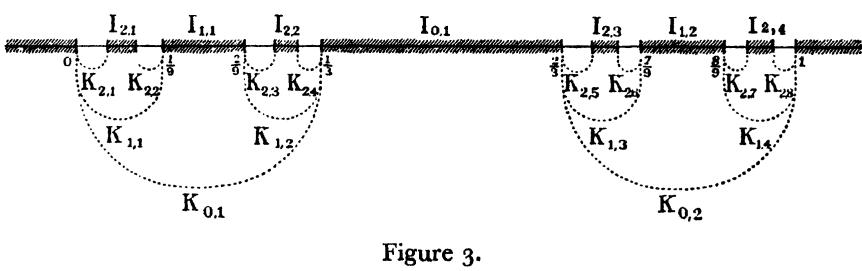
\includegraphics[keepaspectratio]{images/part002_c6c4994f.jpg}}\\
图 3。
若 \(\mathbf{K}'\) 是诸 \(\mathbf{I}_{n,p}\) 的并的余集，则闭集 \(\mathbf{K} = \mathbf{A} \cap \mathbf{K}'\) 称为 Cantor 三分集。显然 \(\mathbf{K}\) 是紧的（第 2 目，定理 2）；而且 \(\mathbf{K}\) 是全不连通的。因为若 \(\mathbf{K}\) 包含一个长度 \(>0\) 的区间 I，则 I 将含于某个区间 \(\mathbf{K}_{m,p}\) ；于是它的长度将 \(\leqslant 1/3^{m+1}\) 对每个 \(m\) 成立，这是荒谬的。

\subsection{区间到区间上的同胚}

定理 5. 设 I 是 R 中的一个区间。则 I 到 R 中的映射 f 是 I 到 \(f(I)\) 上的一个同胚，当且仅当 f 在 I 上严格单调且连续；此时 \(f(I)\) 是 R 中的一个区间。

\begin{enumerate}
\def\labelenumi{\arabic{enumi})}
\tightlist
\item
  条件是必要的。设 \(a\) 与 \(b\) 是 \(I\) 中满足 \(a < b\) 的两点，且例如设 \(f(a) < f(b)\) 。我们来证明 \(f\) 在 \(I\) 上严格递增。首先，若 \(a < c < b\) ，则必有 \(f(a) < f(c) < f(b)\) ；因为若例如有 \(f(a) < f(b) < f(c)\)
\end{enumerate}

则区间 \([a, c]\) 在 \(f\) 下的像将是一个连通集（第一章 § 11 第 2 目，命题 4），从而将包含区间 \([f(a), f(c)]\) ；于是将存在 \(x \in [a, c]\) 使得 \(f(x) = f(b)\) ，与 \(f\) 是单射的假设相矛盾。

由此推出，若 \(x\) 与 \(y\) 是 \(I\) 中满足 \(x < y\) 的任意两点，则 \(f(x) < f(y)\) ；因为 \(f(a) < f(x) < f(b)\) （当 \(a < x < b\) ），\(f(a) < f(b) < f|(x)\) （当 \(b < x\) ），且 \(f(x) < f(a) < f(b)\) （当 \(x < a\) ）；以 \(a, x, y\) 分别代替 \(a, b, x\) 重复上述论证，即见 \(f(x) < f(y)\) 。

\begin{enumerate}
\def\labelenumi{\arabic{enumi})}
\setcounter{enumi}{1}
\tightlist
\item
  条件是充分的。设 \(f\) 在 \(I\) 上连续且严格单调（比如说严格递增）：\(f(I)\) 连通，因而是区间；又因 \(f\) 严格递增，\(f\) 是 \(I\) 到 \(f(I)\) 上的一个双射。此外，\(f\) 把 \(I\) 中的每个开区间映到 \(f(I)\) 中的一个开区间，因此（§ 1 第 4 目，命题 5）\(f\) 是 \(I\) 到 \(f(I)\) 上的一个同胚。
\end{enumerate}

注. 上面证明的第一部分实际上表明，I 到 R 中的连续单射是严格单调的；因此由证明的第二部分推出，区间 I 到 R 中的每个连续单射 f 都是 I 到 \(f(\mathbf{I})\) 上的同胚。

\section{实数域}

\subsection{R 中的乘法}

有理直线 \(\mathbf{Q}\) 的拓扑不仅与加法群结构相容，而且与 \(\mathbf{Q}\) 的域结构相容。因为函数 \(xy\) 在 \((0, 0) \in \mathbf{Q} \times \mathbf{Q}\) 处连续，这是由于对每个整数 \(n > 0\) ，关系 \(|x| \leqslant 1/n\) 与 \(|y| \leqslant 1/n\) 合起来蕴含 \(|xy| \leqslant 1/n^2 \leqslant 1/n\) ；另一方面，若 \(a\) 是任一非零有理数，则函数 \(ax\) 在 \(x = 0\) 处连续，这是由于对每个整数 \(n > 0\) ，关系 \(|x| \leqslant 1/n |a|\) 蕴含 \(|ax| \leqslant 1/n\) 。这表明 \(xy\) 在 \(\mathbf{Q} \times \mathbf{Q}\) 的每一点连续（第三章 § 6 第 3 目）。

为了证明 \(1 / x\) 在 \(\mathbf{Q}^*\) 上连续，我们更精确地证明：\(1 / x\) 在 0 的任一邻域 \(\mathbf{V}\) 的余集中（关于加法结构）一致连续。即我们有 \(\left|\frac{1}{x} - \frac{1}{y}\right| = \frac{|x - y|}{xy}\) ；存在整数 \(m > 0\) ，使得 \(|x| \geqslant 1 / m\) 对每个 \(x \in \mathbb{C}\mathbf{V}\) 成立；若 \(x\) 与 \(y\) 是 \(\mathbb{C}\mathbf{V}\) 中满足 \(|x - y| \leqslant 1 / m^2 n\) 的任意两点，则将有 \(\left|\frac{1}{x} - \frac{1}{y}\right| \leqslant \frac{1}{n}\) 。

在函数 \(1 / x\) 下，\(\mathbf{Q}^*\) 上（关于加法一致结构）的任一不以 \(0\) 为聚点的 Cauchy 滤子的像是（关于加法一致结构的）一个 Cauchy 滤子。因此（第三章 § 6 第 8 目，命题 7）：

命题 1. 分别定义在 Q × Q 与 Q* 上的函数 xy 与 1/x 可以分别连续延拓到 R × R 与 R* 上，并在 R 上定义一个域结构。赋有这个结构的 R 称为实数域。

第三章 § 6 中建立的拓扑域的所有性质当然都适用；特别地，每个以实数为系数的 n 个实变量的有理函数，在其分母不为零的 \(R^{n}\) 的每一点处连续。

\subsection{乘法群 R*}

由第三章 § 6 第 7 目可知，实直线的拓扑在 \(\mathbf{R}^*\) 上诱导的拓扑与 \(\mathbf{R}^*\) 的乘法群结构相容；由于 \(\mathbf{R}^*\) 是局部紧空间 \(\mathbf{R}\) 的开子集，由此推出 \(\mathbf{R}^*\) 是局部紧拓扑群（第一章 § 9 第 7 目，命题 13），因而是完备的（第三章 § 3 第 3 目，命题 4 的推论 1；这也可由第三章 § 6 第 8 目的命题 8 得出）；当然，这后一性质涉及的是 \(\mathbf{R}^*\) 上的乘法一致结构，而不是 \(\mathbf{R}^*\) 上由 \(\mathbf{R}\) 的加法一致结构诱导的一致结构。

函数 \(xy\) 把集 \(\mathbf{Q}_{+} \times \mathbf{Q}_{+}\) 映入 \(\mathbf{Q}_{+}\) ，因此它把 \(\mathbf{R}_{+} \times \mathbf{R}_{+}\) 映入 \(\mathbf{R}_{+}\) （第一章 § 2 第 1 目，定理 1）；换句话说，两个 \(\geqslant 0\) 的实数之积 \(\geqslant 0\) 。于是公式 \((-x)y = -xy\) 与 \((-x)(-y) = xy\) 表明，一个 \(\geqslant 0\) 的数与一个 \(\leqslant 0\) 的数之积 \(\leqslant 0\) ，而两个 \(\leqslant 0\) 的数之积 \(\geqslant 0\) ；由此推出

\[
| x y | = | x |. | y |\tag{1}
\]

（它也可以由 \(\mathbf{Q} \times \mathbf{Q}\) 上相应关系的延拓得到）。

若 \(x > 0\) 且 \(y > 0\) ，我们有 \(xy \neq 0\) ，因而 \(xy > 0\) ；同样，若 \(x < 0\) 且 \(y > 0\) ，则 \(xy < 0\) ；若 \(x < 0\) 且 \(y < 0\) ，则 \(xy > 0\) 。特别地，若 \(x \neq 0\) ，我们有 \(x^2 > 0\) ，因此实数的平方和除非每个数都为零，否则不可能为零。

若 \(x > 0\) 且 \(y \leqslant z\) （相应地 \(y < z\) ），我们有 \(xy \leqslant xz\) （相应地 \(xy < xz\) ）；换句话说，比率 \(> 0\) 的位似保持 \(\mathbf{R}\) 上的次序。由于 \((-x)y = -xy\) ，比率 \(< 0\) 的位似把 \(\mathbf{R}\) 上的序变为反序。

若 \(x > 0\) ，我们有 \(\mathbf{1} / x > 0\) ，因为 \(x.(\mathbf{1} / x) = \mathbf{1} > 0\) 。若 \(0 < x < y\) ，我们有 \(xy > 0\) ，于是 \(x.(\mathbf{1} / xy) < y.(\mathbf{1} / xy)\) ，即 \(\mathbf{1} / y < \mathbf{1} / x\) 。因此，映射 \(x \to \mathbf{1} / x\) 把集 \(\mathbb{R}_+^*\) （即 \(> 0\) 的实数组成的集）映到其自身上，它是严格递减的。

我们同样看出，函数 \(\mathbf{1} / x\) 在 \(] \leftarrow, o[, \text{ 且因此函数 } \frac{\mathbf{1}}{x - a}\) 在区间 \(] \leftarrow, a[ \text{ 与 } ]a, \rightarrow [.\) 的每一个内严格递减。

由上文推出，\(R_{+}^{*}\) 是乘法群 \(R^{*}\) 的一个子群；而且，序关系 \(x \leqslant y\) 与 \(R_{+}^{*}\) 的乘法群结构相容；换句话说，\(R_{+}^{*}\) 是一个全序群。

两个 \(\geqslant0\) 的实数之积 \(\geqslant0\) 这一事实可以表述为：R 是一个有序域；上述所有性质对一切有序域都成立。

命题 2. 乘法群 \(\mathbf{R}^{*}\) （ \(\neq 0\) 的实数组成的）是一个拓扑群，同构于它的子群 \(\mathbf{R}_{+}^{*}\) 与 \(\mathbf{U}_{0}\) 的积，其中

\[
\mathrm{U} _ {0} = \{- 1, + 1 \}.
\]

对每个 \(x \neq 0\) ，令 \(\operatorname{sgn} x\) 表示 \(\frac{x}{|x|}\) （ \(x\) 的符号）。函数 \(\operatorname{sgn}\) 是 \(\mathbf{R}^*\) 到 \(U_0\) 上的一个同态。我们有 \(x = |x| \operatorname{sgn} x\) ，且 \(x\) 的这个表成 \(\mathbf{R}_+^*\) 的一个元素与 \(U_0\) 的一个元素之积的分解是唯一的；因而 \(\mathbf{R}^*\) 的群结构是 \(\mathbf{R}_+^*\) 与 \(U_0\) 的群结构之积。另一方面，映射 \(x \to |x|\) 连续，且 \(x \to \operatorname{sgn} x = \frac{x}{|x|}\) 也连续，因为 \(x \neq 0\) 。由此即得结论。

我们通过令 sgn o = o 把函数 sgn 延拓到整个 R。

我们将在第五章（§ 4 第 1 目，定理 1）看到，拓扑群 \(\mathbf{R}_{+}^{*}\) 同构于加法群 \(\mathbf{R}\) ；这将完成对拓扑群 \(\mathbf{R}^{*}\) 的结构的确定。

\subsection{n 次根}

设 \(n\) 是任一整数 \(> 0\) 。由关系 \(0 < x < y\) ，对 \(n\) 用归纳法推出 \(0 < x^n < y^n\) 。换句话说，函数 \(x \to x^n\) 对 \(x \geqslant 0\) 严格递增；它显然在每一点连续，因此（§ 2 第 6 目，定理 5）是 \(\mathbf{R}_{+}\) 到一个区间 \(\mathbf{I}\) 上的同胚。另一方面，由于 \(x \geqslant 1\) 蕴含 \(x^{n-1} \geqslant 1\) ，从而 \(x^n \geqslant x\) ，可见 \(\mathbf{I}\) 不是有界的，因而 \(\mathbf{I} = \mathbf{R}_{+}\) 。对于 \(x \geqslant 0\) ，映射 \(x \to x^n\) 的逆的值记作 \(x^{1/n}\) 或 \(\sqrt[n]{x}\) ，称为 \(x\) 的 \(1\) 次幂或 \(x\) 的 n 次根（当 \(n = 2\) , 3 时，我们说平方根、立方根；当 \(n = 2\) 时，我们用 \(\sqrt{x}\) 代替 \(\sqrt[2]{x}\) 书写）。正数 \(x^{1/n}\) 于是定义为方程的唯一正解

\[
y ^ {n} = x \quad (x \geqslant 0).\tag{2}
\]

特别地，我们看到存在实数 x 使得 \(x^{2}=2\) ，而没有有理数具有这一性质；这样我们重新得到有理直线 Q 不是完备空间这一事实。

映射 \(x \to x^{1/n}\) （ \(\mathbf{R}_+\) 到其自身的）严格递增且连续。由 (2) 我们有 \(0^{1/n}=0, 1^{1/n}=1\) ，还有

\[
(x y) ^ {1 / n} = x ^ {1 / n} y ^ {1 / n};\tag{3}
\]

因而 \(x \to x^{1/n}\) 是拓扑群 \(\mathbf{R}_{+}^{*}\) 的一个自同构。

在第五章 § 4 第 1 目中，我们将通过求出乘法群 \(\mathbf{R}_{+}^{*}\) 的所有自同构来推广这一结果。

\section{扩充实直线}

\subsection{R 的开区间之间的同胚}

命题 1. \(\mathbf{R}\) 的所有非空开区间都同胚于 \(\mathbf{R}\) 。先考察有界开区间 \(\mathbf{I} = ]a\) , \(b[(a < b)\) 。对每个 \(x \in \mathbf{I}\) ，令 \(f(x) = -\left(\frac{1}{x - a} + \frac{1}{x - b}\right)\) 。这个函数在 \(\mathbf{I}\) 上连续且严格递增，因为我们已看到 \(\frac{1}{x - b}\) 在 \(]\leftarrow, b[\) 中严格递减，而 \(\frac{1}{x - a}\) 在 \(]a, \rightarrow[\) 中严格递减。由此推出 \(f\) 是 \(\mathbf{I}\) 到一个区间 \(f(\mathbf{I})\) （ \(\mathbf{R}\) 中的）上的同胚（ \(\S 2\) 第 6 目，定理 5）。\(f(\mathbf{I})\) 既不上有界也不下有界；因为若例如 \(f(x) \leqslant c\) 对所有 \(x \in \mathbf{I}\) 成立，则将得出 \(1 - \frac{b - x}{x - a} \leqslant c(b - x)\) （因为 \(b - x > 0\) ）；而当 \(x\) 充分接近 \(b\) 时这就导致矛盾（利用不等式两边这两个有理函数在点 \(b\) 处的连续性）。因而 \(f(\mathbf{I}) = \mathbf{R}\) ，从而每个有界开区间都同胚于 \(\mathbf{R}\) 。设 \(g\) 为 \(f\) 的逆：它把 \(\mathbf{R}\) 的每个无界开区间映到一个区间 \(J\) （含于 \(I\) 且在 \(I\) 中开的）上。由于 \(I\) 在 \(\mathbf{R}\) 中开，\(J\) 在 \(\mathbf{R}\) 中也开；由于它有界，它同胚于 \(\mathbf{R}\) ；这样我们就证明了每个无界开区间都同胚于 \(\mathbf{R}\) 。

注. 为了证明所有有界开区间彼此同胚，只需注意：若 \(a \neq b\) 且 \(a' \neq b'\) ，则存在 R 到其自身的一个形如 \(x \to \alpha x + \beta\) 的同胚（且只有一个），它把 a 映到 \(a'\) ，把 b 映到 \(b'\) ，从而把以 a, b 为端点的开（相应地半开、闭）区间映到以 \(a', b'\) 为端点的开（相应地半开、闭）区间；读者通过计算 \(\alpha\) 与 \(\beta\) 容易验证这一点。

\subsection{扩张直线}

我们现在要通过给 R 添加两个新元素来定义一个拓扑空间 \(\overline{R}\) ，使得 R 到 R 的有界开区间 I 上的每个同胚都能延拓为 \(\overline{R}\) 到与 I 有相同端点的闭区间上的同胚。

设 \(\overline{\mathbf{R}}\) 是由（集合论， R, § 4 第 5 目）向 \(\mathbf{R}\) 添加两个新元素得到的集，这两个新元素记作 \(-\infty\) 与 \(+\infty\) 。我们通过把 \(\mathbf{R}\) 上的序延拓到 \(\overline{\mathbf{R}}\) ，方式是令 \(-\infty < a\) 与 \(a < +\infty\) （对所有 \(a \in \mathbf{R}\) ）以及 \(-\infty < +\infty\) ；显然我们如此得到一个全序集，其序在 \(\mathbf{R}\) 上诱导出实直线的序。其次，考察 \(\overline{\mathbf{R}}\) 上由 \(\overline{\mathbf{R}}\) 的开区间全体所生成的拓扑。由于在 \(\mathbf{R}\) 上 \(\overline{\mathbf{R}}\) 的开区间的迹是 \(\mathbf{R}\) 的开区间，这个拓扑在 \(\mathbf{R}\) 上诱导出实直线的拓扑。

定义 1. 赋有上述序结构与拓扑的集合 \(\overline{\mathbf{R}}\) 称为扩充实直线。

在使用扩张直线 \(\overline{\mathbf{R}}\) 时，出于用语习惯，把它的点称为实数往往是方便的；这时 \(\mathbf{R}\) 的点称为有限实数。我们在本节及本章随后三节中采用这一约定；今后凡采用这一约定时，我们都会明确指出它适用于正文的哪一部分。

若 \(a\) 是有限实数，则区间 \([a, +\infty[ \text{ 与 } ] - \infty, a]\) （相应地 \(]a, +\infty[ \text{ 与 } ] - \infty, a[\) ）（ \(\overline{\mathbf{R}}\) 中的）含于 \(\mathbf{R}\) ，且与 \(\mathbf{R}\) 中迄今记作 \([a, \rightarrow[ \text{ 与 } ] \leftarrow, a]\) （相应地 \(]a, \rightarrow[ \text{ 与 } ] \leftarrow, a[\) ）的区间一致；这个新记号用得远为频繁。再者，\(\mathbf{R}\) 与区间 \(] - \infty, +\infty[ \text{ 位于 } \overline{\mathbf{R}}, \text{ 且有时也如此记之。}\)

命题 2. 每个同胚 \(f\) （ \(\mathbf{R}\) 到区间 \(]a, b[\) 上的）都可以延拓为同胚 \(\overline{f}\) （ \(\overline{\mathbf{R}}\) 到 \([a, b]\) 上的）。若 \(f\) 是递增函数，则 \(\overline{f}\) 是 \(\overline{\mathbf{R}}\) 到 \([a, b]\) 上的一个序同构。

设 \(f\) 是递增同胚。若把 \(f\) 延拓到 \(\mathbf{R}\) ，方式是令 \(\overline{f}(-\infty) = a\) 与 \(\overline{f}(+\infty) = b\) ，则显然 \(\overline{f}\) 是 \(\overline{\mathbf{R}}\) 到 \([a, b]\) 上的严格递增映射（因而是双射）。于是 \(\overline{f}\) 把 \(\overline{\mathbf{R}}\) 的每个开区间映到关于 \([a, b]\) 为开的一个区间，因而由 § 1 第 4 目的定义 1 与命题 5，它是 \(\overline{\mathbf{R}}\) 到 \([a, b]\) 上的同胚。

若 \(f\) 递减，则对递增同胚 \(x \to -f(x)\) （ \(\mathbf{R}\) 到 \(] - b, - a[\) 上的）应用已证的结果。

因此，§ 2 中得到的区间 \([a, b]\) 的所有只涉及区间的序结构与拓扑的性质都可以搬到 \(\overline{R}\) 上；于是有下列命题：

命题 3. 扩充实直线是紧的。

因此（第二章 § 4 第 1 目，定理 1）在 \(\overline{\mathbf{R}}\) 上存在唯一一个与其拓扑相容的一致结构；这个一致结构同构于在 \([a, b]\) 上由 \(\mathbf{R}\) 的加法一致结构诱导的一致结构。但应当注意，在 \(\mathbf{R}\) 上由 \(\overline{\mathbf{R}}\) 的一致结构诱导的一致结构不是 \(\mathbf{R}\) 的加法一致结构（尽管它与实直线的拓扑相容）；因为 \(\mathbf{R}\) 关于其加法一致结构是完备空间，却不是 \(\overline{\mathbf{R}}\) 的完备子空间，因为它在 \(\overline{\mathbf{R}}\) 中不闭。

命题 4. \(\overline{\mathbf{R}}\) 的每个非空子集都有上确界与下确界。

R 的非空子集 A 的上确界（相应地下确界）记作 sup A（相应地 inf A）。显然

\[
\inf A \leqslant \sup A.\tag{1}
\]

若 \(\mathbf{A} \subset \mathbf{B}\) ，则 \(\sup \mathbf{A} \leqslant \sup \mathbf{B}\) 且 \(\inf \mathbf{A} \geqslant \inf \mathbf{B}\) （集合论，第三章 § 1 第 9 目，命题 4）。

命题 5. \(\overline{R}\) 的子集 A 连通当且仅当 A 是区间。

推论. 扩充实直线是连通的、局部连通的空间。

命题 6. 映射 \(f\) （区间 \(I\) （ \(\overline{R}\) 的）到 \(\overline{R}\) 中的）是 \(I\) 到 \(f(I)\) 上的同胚，当且仅当 \(f\) 在 \(I\) 上严格单调且连续；此时 \(f(I)\) 是 \(\overline{R}\) 的一个区间。

最后，函数 \(\sup (x,y)\) 与 \(\inf (x,y)\) 在 \(\overline{\mathbf{R}}\times \overline{\mathbf{R}}\) 上连续

\subsection{\texorpdfstring{\(\bar{R}\) 中的加法与乘法}{\textbackslash bar\{R\} 中的加法与乘法}}

首先注意，函数 \(-x\) 可以连续延拓到 \(\overline{\mathbf{R}}\) ，依照公式 \(-(-\infty)=+\infty\) 与 \(-(+\infty)=-\infty\) ；如此延拓后的函数是 \(\overline{\mathbf{R}}\) 到其自身的一个同胚。

其次，考察函数 \(x + y\) 与 xy，它们定义在 \(R \times R\) 上、取值于 R 中；通过认为它们取值于拓扑空间 \(\overline{R}\) ，我们将看到它们也能在 \(\overline{R} \times \overline{R}\) 的某些点连续延拓。

就 \(x + y\) 而言，令 \(A' = ] - \infty, + \infty]\) 与 \(A'' = [-\infty, + \infty[\) 。于是有下述命题：

命题 7. 函数 \(x + y\) 可以依照公式连续延拓到集 \(\mathbf{A}' \times \mathbf{A}'\) 与 \(\mathbf{A}'' \times \mathbf{A}''\) 的每一个上，公式为

\[
\left\{ \begin{array}{l l} x + (+ \infty) = (+ \infty) + x = + \infty & (x \neq - \infty), \\ x + (- \infty) = (- \infty) + x = - \infty & (x \neq + \infty). \end{array} \right.\tag{2}
\]

例如我们证明：当 \((x,y)\) 趋于点 \((a,+\infty)\) \((a\neq-\infty)\) 而保持属于 \(R\times R\) 时，\(x+y\) 趋于 \(+\infty\) 。存在有限数 b\textless a ，而区间 {]}b, \(+\infty\) {[} 是 a 在 R 中的邻域；对任意有限 c ，关系 x\textgreater b 与 y\textgreater c-b 蕴含 \(x+y>c\) ，这表明 \(x+y\) 可以任意接近 \(+\infty\) ，只要 \((x,y)\) 充分接近 \((a,+\infty)\) 。其他情形论证类似。

相反，\(x + y\) 在点 \((-\infty, +\infty)\) 与 \((+\infty, -\infty)\) （ \(\overline{\mathbf{R}} \times \overline{\mathbf{R}}\) 的）处没有极限。因为若 \(x + y\) 有极限 \(k\) （有限或无限），当 \((x, y)\) 趋于 \((+\infty, -\infty)\) 而保持属于 \(\mathbf{R} \times \mathbf{R}\) 时，则将推出：对每个有限 \(a\) ，函数 \((x + a) - x\) 将趋于 \(k\) ，当 \(x\) 趋于 \(+\infty\) 而保持属于 \(\mathbf{R}\) 时；而这是荒谬的，因为 \((x + a) - x = a\) 且 \(a\) 是任意的。

函数 \(x + y\) 把 \(A' \times A'\) （相应地 \(A'' \times A''\) ）映入 \(A'\) （相应地 \(A''\) ）。因此它是 \(A'\) （相应地 \(A''\) ）上的一个合成法则，它延拓了 \(R\) 上的加法法则。由恒等延拓原理（第一章 § 8 第 1 目，命题 2 的推论 1），这个法则交换且结合； o 是这个法则的单位元素；而由公式 (2)，\(A'\) 的唯一非正则元素（代数，第一章 § 2 第 2 目）是 \(+\infty\) 。

若 \(x, y, z, t\) 是 \(\overline{\mathbf{R}}\) 中满足 \(x \leqslant y\) 与 \(z \leqslant t\) 的点，则只要不等式两边都有定义，就有 \(x + z \leqslant y + t\) 。

注意在 \(\overline{\mathbf{R}}\) 中，由公式 (2)，关系 \(x < y\) 蕴含 \(x + z < y + z\) 仅当 \(z\) 有限时；容易验证，只要不等式两边都有定义，关系 \(x < y\) 与 \(z < t\) 就蕴含 \(x + z < y + t\) 。

在 \(\overline{\mathbf{R}}\) 中我们令 \(x^{+} = \sup (x,0)\) ，\(x^{-} = \sup (-x,0)\) ，\(|x| = \sup (x, - x)\) ；于是 \((+\infty)^{+} = (-\infty)^{-} = +\infty\) 且 \((+\infty)^{-} = (-\infty)^{+} = 0\) ，而 \(|+\infty| = |- \infty| = +\infty\) 。和 \(x^{+} - x^{-}\) 与 \(x^{+} + x^{-}\) 对所有 \(x \in \overline{\mathbf{R}}\) 有定义，因而由恒等延拓原理分别等于 \(x\) 与 \(|x|\) 。同样，只要和 \(x + y\) 有定义，我们就有 \(|x + y| \leqslant |x| + |y|\) 。

相反要注意，§ 1 第 1 目的公式 (6) 与 (7) 对某些值 \(x\) 与 \(y\) （ \(\overline{\mathbf{R}}\) 中的）可能不再有意义；例如，若 \(x = -\infty\) 且 \(y = 0\) ，我们有 \(\sup (x, y) = 0\) ，但和 \(x + (y - x)^+\) 没有定义，因为 \((y - x)^+ = +\infty\) 。

令 \(\overline{\mathbf{R}}^{*}\) 表示 \(o\) 在 \(\overline{\mathbf{R}}\) 中的余集。于是乘法情形的命题 7 的类似命题如下：

命题 8. 函数 \(xy\) 可以依照公式连续延拓到集 \(\overline{\mathbf{R}}^* \times \overline{\mathbf{R}}^*\) 上，公式为

\[
\left\{ \begin{array}{l} x. (+ \infty) = (+ \infty). x = \left\{ \begin{array}{l l} + \infty & \text {if} \quad x > 0 \\ - \infty & \text {if} \quad x <   0 \end{array} \right. \\ x. (- \infty) = (- \infty). x = \left\{ \begin{array}{l l} - \infty & \text {if} \quad x > 0 \\ + \infty & \text {if} \quad x <   0. \end{array} \right. \end{array} \right.\tag{3}
\]

我们把证明留给读者；它与命题 7 的证明类似。

同样，我们看到 \(xy\) 在点 \((0, +\infty), (+\infty, 0), (0, -\infty), (-\infty, 0)\) （ \(\overline{\mathbf{R}} \times \overline{\mathbf{R}}\) 的）处没有极限。

函数 \(xy\) 是 \(\overline{\mathbf{R}}^*\) 上的一个合成法则，它延拓了 \(\mathbf{R}\) 上的乘法法则；这个法则结合且交换（恒等延拓原理）；它以 1 为单位元素；而 \(\overline{\mathbf{R}}^*\) 中的非正则元素是 \(+\infty\) 与 \(-\infty\) 。

若 \(x \leqslant y\) 且 \(z > 0\) ，则只要不等式两边都有定义，就有 \(xz \leqslant yz\) 。若积 \(xy\) 有定义，则 \(|x| \cdot |y|\) 也有定义，且我们有 \(|xy| = |x| \cdot |y|\) 。

最后，分配律公式

\[
x (y + z) = x y + x z\tag{4}
\]

只要出现在两边的所有运算都有定义，它由恒等延拓原理仍然有效。

\pandocbounded{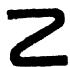
\includegraphics[keepaspectratio]{images/part002_cca5eabe.jpg}}

注意可能发生 (4) 的左边有定义而右边没有定义的情形：例如考察 \(x = +\infty\) ， y = 2 与 z = -1 的情形。因此在 R 中使用分配律公式应当谨慎。

\section{实值函数}

\subsection{实值函数}

定义 1. 一个集 X 到实直线中的映射称为定义在 X 上的实值函数（或实函数）。

通过与 § 4 第 2 目所述类似的用语习惯，X 到 \(\overline{\mathbf{R}}\) 中的映射在本节及下一节中也称为定义在 X 上的实值函数。X 到 \(\mathbf{R}\) 中的映射将称为有限实值函数。

若 \(f\) 与 \(g\) 是定义在 \(\mathbf{X}\) 上的两个实值函数，则关系 \(f \leqslant g\) 依定义等价于“\(f(x) \leqslant g(x)\) 对所有 \(x \in \mathbf{X}\) 成立；”这个关系是集 \(\overline{\mathbf{R}}^{\mathbf{X}}\) （ \(\mathbf{X}\) 上所有实值函数的）上的一个序。由这个关系排序的集 \(\overline{\mathbf{R}}^{\mathbf{X}}\) 是一个格；因为若 \(f\) 与 \(g\) 是任意两个实值函数，则函数 \(h\) 由 \(h(x) = \sup (f(x), g(x))\) （对所有 \(x \in \mathbf{X}\) ）所定义，它是 \(\mathbf{X}\) 上既 \(\geqslant f\) 又 \(\geqslant g\) 的实值函数中的最小者；按照一般记号，我们把这个函数（即 \(f\) 与 \(g\) 在 \(\overline{\mathbf{R}}^{\mathbf{X}}\) 中的上确界）记作 \(\sup (f, g)\) 。类似地，在每个 \(x \in \mathbf{X}\) 处取值 \(\inf (f(x), g(x))\) 的函数记作 \(\inf (f, g)\) 。

注意 sup \((f, g)\) 是映射

\[
(u, v) \mapsto \sup (u, v)
\]

\(\overline{\mathbf{R}}\times \overline{\mathbf{R}}\) 到 \(\overline{\mathbf{R}}\) 中的映射与映射 \(x\to (f(x),g(x))\) （ \(\mathbf{X}\) 到 \(\overline{\mathbf{R}}\times \overline{\mathbf{R}}\) 中的）的复合。inf \((f,g)\) 亦然。

实值函数 \(f\) （定义在集 \(\mathbf{X}\) 上的）称为在 \(\mathbf{X}\) 中上有界（相应地下有界）的，如果 \(f(\mathbf{X})\) 是 \(\mathbf{A}'' = [-\infty, +\infty[\) 的子集且上有界（相应地，如果 \(f(\mathbf{X})\) 是 \(\mathbf{A}' = ] - \infty, +\infty]\) 的子集且下有界）。\(f\) 称为在 \(\mathbf{X}\) 中有界的，如果它既上有界又下有界，也就是说 \(f(\mathbf{X})\) 是 \(\mathbf{R}\) 的有界子集。

因此每个有界函数都是有限的。其逆不真，例如函数 \(\mathbf{1} / x\) （在 \(\mathbb{R}_+^* = ]0, +\infty[\) 上）所示。
